\documentclass[12pt, a4paper, twoside, openany]{book}

% ── Codificación y lengua ────────────────────────────────────────────────────
\usepackage[T1]{fontenc}
\usepackage[utf8]{inputenc}
\usepackage[british]{babel}

% ── Tipografía ───────────────────────────────────────────────────────────────
\usepackage{palatino}
\usepackage{microtype}

% ── Títulos de capítulo y sección ────────────────────────────────────────────
\usepackage{titlesec}
\titleformat{\chapter}[display]
  {\normalfont\huge\bfseries}
  {\large\chaptertitlename\ \thechapter}
  {8pt}
  {\Huge}
\titlespacing*{\chapter}{0pt}{-10pt}{30pt}

% ── Márgenes ─────────────────────────────────────────────────────────────────
\usepackage[top=3cm, bottom=3cm, left=3.5cm, right=2.5cm]{geometry}

% ── Gráficos y colores ───────────────────────────────────────────────────────
\usepackage{graphicx}
\usepackage{subcaption}
\usepackage{xcolor}
\graphicspath{{figures/}}

% ── Tablas ───────────────────────────────────────────────────────────────────
\usepackage{booktabs}
\usepackage{longtable}
\usepackage{multirow}

% ── Matemáticas ──────────────────────────────────────────────────────────────
\usepackage{amsmath}
\usepackage{amssymb}
\usepackage{eurosym}

% ── Código fuente ────────────────────────────────────────────────────────────
\usepackage{listings}
\lstset{
  basicstyle=\ttfamily\small,
  breaklines=true,
  frame=single,
  numbers=left,
  numberstyle=\tiny,
  language=Python
}

% ── Hipervínculos ────────────────────────────────────────────────────────────
\definecolor{navyblue}{RGB}{0,32,96}
\usepackage[
  colorlinks  = true,
  linkcolor   = navyblue,   % refs internas: tablas, figuras, secciones
  citecolor   = navyblue,   % citas bibliográficas
  urlcolor    = navyblue,   % URLs
  filecolor   = navyblue
]{hyperref}
\usepackage{url}

% ── Cabeceras y pies de página ───────────────────────────────────────────────
\usepackage{fancyhdr}
\setlength{\headheight}{15pt}   % evita el aviso "headheight too small" de fancyhdr
\setlength{\emergencystretch}{3em}  % reduce los overfull \hbox cosméticos
\pagestyle{fancy}
\fancyhf{}
% Páginas pares: nombre del máster (izq.); impares: capítulo (der.).
% Se separan por paridad de página para que los dos textos nunca coincidan ni se solapen.
\fancyhead[LE]{\footnotesize\textsc{MSc. Modelling for Science and Engineering}}
\fancyhead[RO]{\footnotesize\textsc{\leftmark}}
\renewcommand{\chaptermark}[1]{\markboth{#1}{}}
\renewcommand{\headrulewidth}{0.4pt}
% Abajo izquierda: número de página
\fancyfoot[R]{\small\thepage}
% Páginas de inicio de capítulo: solo número abajo derecha
\fancypagestyle{plain}{
  \fancyhf{}
  \fancyfoot[R]{\small\thepage}
  \renewcommand{\headrulewidth}{0pt}
}

% ── Pies de figura/tabla ─────────────────────────────────────────────────────
\usepackage{caption}
\captionsetup{font=small, labelfont=bf, labelsep=period}

% ── Cajas para destacar hallazgos clave ──────────────────────────────────────
\usepackage[most]{tcolorbox}
\newtcolorbox{hallazgo}{
  colback=navyblue!4, colframe=navyblue!55, boxrule=0.6pt, arc=2pt,
  left=8pt, right=8pt, top=6pt, bottom=6pt,
  fonttitle=\bfseries\small, title={Key finding}
}

% ── Bibliografía ─────────────────────────────────────────────────────────────
\usepackage{csquotes}   % recomendado por biblatex con babel
\usepackage[backend=biber, style=numeric, sorting=none]{biblatex}
\addbibresource{bibliography.bib}

% ── Metadatos ────────────────────────────────────────────────────────────────
\title{Integrated Machine Learning for ROI Optimization: From Hierarchical Propensity Modeling to Time-Series Forecasting with Prophet}
\author{Germán}
\date{2026}

% ════════════════════════════════════════════════════════════════════════════
\begin{document}

\frontmatter
\begin{titlepage}
  \centering
  \vspace*{2cm}

  {\LARGE \textbf{Trabajo de Fin de Máster}\par}
  \vspace{0.5cm}
  {\large Master's Degree in Modelling for Science and Engineering\\
  Data Science Specialization\par}
  \vspace{2cm}

  \rule{\linewidth}{0.5mm}
  \vspace{0.4cm}
  {\huge \bfseries Aprendizaje automático para email marketing:\\
  propensión, recomendación y previsión\\
  con validación rigurosa\par}
  \vspace{0.4cm}
  \rule{\linewidth}{0.5mm}

  \vspace{2cm}

  \begin{tabular}{rl}
    \textbf{Autor:}    & Germán Gallego Garcia \\[0.4em]
    \textbf{Director:} & Rubén Campuzano Hernández \\[0.4em]
    \textbf{Fecha:}    & Junio 2026 \\
  \end{tabular}

  \vfill

\end{titlepage}

\chapter*{Resumen}
\addcontentsline{toc}{chapter}{Resumen}

El email marketing es uno de los canales publicitarios digitales con mayor retorno potencial, pero su eficacia depende de la capacidad de dirigirse al usuario adecuado con el mensaje correcto. Las empresas que operan en este canal se enfrentan a un problema de asignación de inversión: ¿qué usuarios tienen mayor probabilidad de interactuar con un producto determinado, y cómo evoluciona esa demanda a lo largo del tiempo?

Este trabajo aborda ese problema mediante un \textit{framework} integral de aprendizaje automático aplicado a campañas reales del mercado español. El pipeline desarrollado cubre desde la ingesta y limpieza de datos hasta la generación de recomendaciones personalizadas, pasando por el enriquecimiento demográfico y geográfico de perfiles de usuario, la segmentación no supervisada de clientes y el modelado de propensión.

El sistema se estructura en cuatro módulos. El primero (M0/M1) realiza dos niveles de segmentación: una segmentación demográfica pura mediante autoencoder y KMeans orientada al arranque en frío, y una segmentación comportamental sobre el historial de interacciones mediante PCA y KMeans. El segundo módulo (M2) desarrolla un modelo de propensión basado en LightGBM que incorpora variables de usuario y de producto ---incluidos \textit{embeddings} del texto del asunto---, con corrección explícita del sesgo de muestreo; se comparan cinco algoritmos (incluida una red neuronal) y dos arquitecturas (un modelo plano frente a uno jerárquico sector\,$\rightarrow$\,producto), y se adopta el modelo plano, que supera al jerárquico en todos los algoritmos. El tercer módulo (M3) implementa un recomendador por cluster: sirve a cada usuario el \textit{ranking} de categorías de su segmento comportamental. El cuarto módulo (M4) aplica el modelo Prophet para la predicción del volumen semanal de clics.

La evaluación se realiza sin fuga de datos (validación agrupada por usuario en M2; partición temporal y reconstrucción del segmento solo con \textit{train} en M3) y con contraste estadístico (intervalos \textit{bootstrap}, Friedman, Wilcoxon y McNemar con corrección de Holm). Un hallazgo central es que la señal útil para la propensión reside en el contenido del producto (PR-AUC, área bajo la curva de precisión-exhaustividad, 0,402 del modelo con variables de producto frente a 0,313 del baseline), mientras que las variables demográficas ---sintéticas--- tienen un poder predictivo limitado. En recomendación, una vez eliminada la fuga, la popularidad es un \textit{baseline} que el segmento no logra batir (Hit~Rate@5 0,586 del recomendador frente a 0,629 de la popularidad); el valor del recomendador por cluster es operativo (interpretabilidad y arranque en frío), no de mejora del \textit{ranking}.

\bigskip
\noindent\textbf{Palabras clave:} email marketing, modelado de propensión, LightGBM, segmentación de usuarios, autoencoder, sistemas de recomendación, enriquecimiento demográfico, corrección de prior shift.

\bigskip\bigskip

\noindent\textbf{Abstract}

\medskip
Email marketing is one of the digital advertising channels with the highest potential return on investment, but its effectiveness depends on the ability to target the right user with the right message. Companies operating in this channel face an investment allocation problem: which users are most likely to engage with a given product, and how does that demand evolve over time?

This thesis addresses that problem through a comprehensive machine learning framework applied to real campaigns from the Spanish market. The developed pipeline covers the full lifecycle from data ingestion and cleaning to personalised recommendations, including demographic and geographic enrichment of user profiles, unsupervised customer segmentation, and propensity modelling.

The system is organised into four modules. The first (M0/M1) performs two levels of segmentation: a purely demographic segmentation via autoencoder and KMeans for cold-start assignment, and a behavioural segmentation over interaction history via PCA and KMeans. The second module (M2) develops a LightGBM propensity model that incorporates both user and product features ---including \textit{embeddings} of the email subject---, with explicit correction of the sampling bias; five algorithms (including a neural network) and two architectures (a flat model vs.\ a hierarchical sector\,$\rightarrow$\,product one) are compared, and the flat model ---which outperforms the hierarchical one across all algorithms--- is adopted. The third module (M3) implements a cluster-level recommender: each user is served the category \textit{ranking} of their behavioural segment. The fourth module (M4) applies the Prophet model for weekly click-volume forecasting. Evaluation is performed without data leakage (user-grouped cross-validation in M2; temporal split and train-only reconstruction of the segment in M3) and with statistical testing (\textit{bootstrap} intervals, Friedman, Wilcoxon and McNemar with Holm correction). A central finding is that the useful signal for propensity lies in product content (PR-AUC 0.402 for the product-aware model vs.\ 0.313 for the baseline), whereas the ---synthetic--- demographic features have limited predictive power. In recommendation, once the leakage is removed, popularity is a baseline the segment fails to beat (Hit~Rate@5 0.586 for the recommender vs.\ 0.629 for popularity); the value of the cluster-level recommender is operational (interpretability and cold-start), not ranking improvement.

\bigskip
\noindent\textbf{Keywords:} email marketing, propensity modelling, LightGBM, user segmentation, autoencoder, recommender systems, demographic enrichment, prior shift correction.

\chapter*{Agradecimientos}
\addcontentsline{toc}{chapter}{Agradecimientos}

% Escribe aquí tus agradecimientos


\tableofcontents
\listoffigures
\listoftables

\mainmatter
\part{Framework and data}
\chapter{Introducción}

\section{Contexto y motivación}

El correo electrónico sobrevive a la proliferación de canales publicitarios por una razón económica: su coste por impacto es bajo y permite ajustar el mensaje al perfil de cada receptor. Esa ventaja, sin embargo, solo se materializa cuando la empresa acierta a quién contactar y con qué producto. Una campaña enviada de forma indiscriminada gasta el mismo presupuesto que una segmentada, pero rinde mucho menos; el problema, por tanto, no es enviar correos, sino decidir bien a quién dirigir cada uno.

En la práctica, los responsables de campaña se enfrentan a un problema de asignación de inversión con información incompleta: el comportamiento real del usuario ante un correo electrónico es difícil de anticipar, y los datos disponibles suelen ser escasos, ruidosos y con un fuerte desbalanceo entre interacciones positivas y negativas. La tasa real de clic en campañas de email marketing se sitúa habitualmente por debajo del 5\%, lo que convierte la predicción de comportamiento en un problema de clasificación con clases muy desbalanceadas.

El aprendizaje automático ofrece herramientas para abordar este problema de forma sistemática, combinando señales de comportamiento pasado con características del usuario y del producto anunciado. No obstante, su aplicación efectiva requiere decisiones metodológicas cuidadosas, especialmente en lo relativo al tratamiento del desbalanceo de clases, la escasez de interacciones observadas y la incorporación de información contextual externa.

\section{Pregunta de investigación y objetivos}

La pregunta central de este trabajo es la siguiente: \textit{¿en qué medida es posible predecir la probabilidad de interacción de un usuario con una campaña de email marketing a partir de su perfil demográfico, su historial de comportamiento y las características del producto anunciado, y qué tipo de señal resulta más determinante?}

Para dar respuesta a esta pregunta, se plantean los siguientes objetivos:

\begin{enumerate}
    \item Construir un pipeline de preprocesado que integre datos de campaña con información geográfica y demográfica de fuentes externas, generando perfiles de usuario completos y homogéneos.
    \item Desarrollar dos niveles de segmentación no supervisada: una segmentación demográfica pura para la asignación de usuarios nuevos (arranque en frío), y una segmentación comportamental basada en el historial de interacciones.
    \item Implementar un modelo de propensión que combine variables de usuario y de producto ---incluido el texto del asunto del correo---, comparando algoritmos y arquitecturas (plano frente a jerárquico), validado sin fuga de datos y con corrección explícita del sesgo de muestreo introducido por el entrenamiento balanceado.
    \item Construir un sistema de recomendación de productos y evaluarlo de forma controlada (partición temporal, \textit{baselines} de referencia y contraste estadístico), determinando qué señal (comportamental o demográfica) resulta más útil para el \textit{ranking}.
    \item Predecir el volumen semanal de clics mediante modelado de series temporales para apoyar la planificación de campañas.
\end{enumerate}

\medskip
\noindent\textbf{Enfoque y contribución.} El énfasis de este trabajo es metodológico. Más que maximizar una métrica de exactitud, se construye un pipeline reproducible de extremo a extremo (del dato bruto a un ejemplo de despliegue) que toma cada decisión de forma justificada: validación sin fuga de datos, comparación de cada modelo frente a \textit{baselines} triviales antes de adoptarlo, corrección del sesgo de muestreo y contraste estadístico de cada afirmación. La aportación no es un predictor de máximo rendimiento, sino un proceso que determina, con evidencia, qué señal es útil, qué modelo merece desplegarse y a qué coste. Por ello varias de las hipótesis siguientes se plantean precisamente para poder ser \emph{refutadas}: el valor del trabajo está tanto en confirmarlas como en descartarlas con fundamento. En suma, este TFM es una guía de cómo abordaría un equipo de datos un proyecto orientado a maximizar el ROI de las campañas: qué construir en cada etapa, cómo validarlo y cómo decidir qué merece desplegarse y qué no. El objeto de estudio es, por tanto, \emph{el método} tanto como los modelos: que algunos resultados sean negativos no resta valor al trabajo, sino que muestra el proceso funcionando como debe.

\medskip
\noindent\textbf{Hipótesis.} A partir de la pregunta y los objetivos, el trabajo contrasta cuatro hipótesis falsables:
\begin{itemize}
    \item \textbf{H1.} Las variables de \emph{producto} (sector, categoría y texto del asunto) mejoran de forma significativa la propensión al clic frente a un modelo que solo usa variables de usuario y frente al \textit{baseline} de popularidad.
    \item \textbf{H2.} Las variables demográficas enriquecidas aportan poder predictivo a la propensión al clic; se contrasta pese a su naturaleza sintética (Capítulo~\ref{cap:datos}), precisamente para medir cuánta señal individual conservan.
    \item \textbf{H3.} Un recomendador basado en el segmento comportamental del usuario supera al \textit{baseline} de popularidad en el \textit{ranking} de productos.
    \item \textbf{H4.} El modelo Prophet mejora la previsión del volumen de clics frente a \textit{baselines} ingenuos (naïve y media móvil).
\end{itemize}
El contraste de cada hipótesis se aborda, respectivamente, en los módulos M2 (Capítulo~\ref{cap:propension}; H1 y H2, esta última vía el estudio de ablación), M3 (Capítulo~\ref{cap:recomendador}; H3) y M4 (Capítulo~\ref{cap:forecast}; H4).

\section{Estructura de la memoria}

La memoria se organiza siguiendo el flujo del pipeline. El capítulo~\ref{cap:estado_arte} revisa el estado del arte en modelado de propensión, segmentación de clientes, sistemas de recomendación y predicción temporal aplicados al marketing digital. El capítulo~\ref{cap:datos} describe las fuentes de datos, el proceso de limpieza, el enriquecimiento demográfico-geográfico y el análisis exploratorio. El capítulo~\ref{cap:evaluacion} ofrece una visión general del pipeline y el marco de evaluación común (métricas, validación sin fuga y pruebas estadísticas). A continuación, cada módulo se presenta en su propio capítulo, exponiendo de forma conjunta su método y sus resultados: segmentación de clientes (Capítulo~\ref{cap:segmentacion}), modelo de propensión (Capítulo~\ref{cap:propension}), recomendador (Capítulo~\ref{cap:recomendador}) y previsión temporal (Capítulo~\ref{cap:forecast}). El capítulo~\ref{cap:negocio} cubre el despliegue de ejemplo y el análisis de retorno de la inversión. Finalmente, el capítulo~\ref{cap:conclusiones} recoge la discusión, las conclusiones y las líneas de trabajo futuro.

\chapter{Estado del arte}
\label{cap:estado_arte}

\section{Email marketing y comportamiento del usuario}

El email marketing es uno de los canales de marketing directo con mayor longevidad en el entorno digital, con un retorno medio de entre 36 y 40 dólares por cada dólar invertido según los informes anuales de la industria \cite{litmus2023}. La literatura coincide en que ese rendimiento depende de la capacidad de segmentar la audiencia y personalizar el mensaje, dos problemas sobre los que se asienta el resto de este capítulo.

El comportamiento del usuario ante un correo electrónico se modela habitualmente mediante tres tipos de evento: impresión (\textit{open}), interacción activa (\textit{click}) y ausencia de respuesta (\textit{ignored}). La tasa de clic sobre impresiones (\textit{click-through rate}, CTR) varía entre el 1\% y el 5\% dependiendo del sector, lo que genera un fuerte desbalanceo de clases que condiciona las decisiones metodológicas en los modelos predictivos \cite{chaffey2024}.

Desde el punto de vista predictivo, los primeros trabajos en este dominio se basaron en modelos logísticos y árboles de decisión aplicados sobre atributos del correo y del receptor \cite{sahni2016}. Con la aparición de métodos de \textit{gradient boosting} y el incremento en la disponibilidad de datos, los enfoques basados en LightGBM \cite{ke2017lightgbm} y XGBoost \cite{chen2016xgboost} se han convertido en el estándar industrial para la predicción de comportamiento en marketing directo, gracias a su capacidad de manejar variables categóricas, datos faltantes y desequilibrios de clase de forma nativa.

\section{Segmentación de clientes}

La segmentación de clientes tiene como objetivo identificar grupos de usuarios con patrones de comportamiento o características demográficas similares, de modo que la comunicación pueda adaptarse a cada grupo. Los métodos de clustering no supervisado más utilizados en este dominio son KMeans \cite{macqueen1967}, modelos de mezcla gaussiana \cite{reynolds2009} y algoritmos de clustering basado en densidad como DBSCAN \cite{ester1996} y su extensión jerárquica HDBSCAN \cite{campello2013}.

La elección del número de clusters es uno de los problemas fundamentales del aprendizaje no supervisado. Los criterios más utilizados son el coeficiente de silueta \cite{rousseeuw1987}, el índice de Calinski-Harabasz \cite{calinski1974} y el índice de Davies-Bouldin \cite{davies1979}, que evalúan la cohesión intra-cluster y la separación inter-cluster desde perspectivas complementarias.

En contextos con alta dimensionalidad, es habitual aplicar técnicas de reducción dimensional previas al clustering. El Análisis de Componentes Principales (PCA) \cite{jolliffe2002} es la técnica lineal más utilizada; los autoencoders \cite{hinton2006} permiten capturar relaciones no lineales que PCA no modela. Trabajos sobre \textit{deep embedded clustering} muestran que las representaciones aprendidas por redes neuronales pueden mejorar el agrupamiento frente a métodos lineales al capturar estructura no lineal de los datos \cite{xie2016}.

Para la visualización de clusters en dos dimensiones, UMAP \cite{mcinnes2018} ha sustituido progresivamente a t-SNE \cite{vandermaaten2008} en la práctica gracias a su mayor velocidad y a la preservación de la estructura global de los datos.

\section{Modelos predictivos en marketing}

\subsection{Modelado de propensión}

El modelado de propensión (\textit{propensity modeling}) consiste en estimar la probabilidad de que un individuo realice una acción de interés —en este caso, hacer clic en un correo— dado su perfil observable. Es una aplicación directa de la clasificación binaria con especial énfasis en la calibración de probabilidades.

Un reto frecuente en este contexto es el sesgo de muestreo: cuando los datos de entrenamiento se construyen con una proporción artificial de positivos y negativos distinta de la distribución real, las probabilidades predichas quedan infladas o defladas respecto al prior verdadero. La corrección de Dal Pozzolo et al. \cite{dalpozzolo2015} proporciona un ajuste exacto en log-odds para recuperar probabilidades calibradas respecto al prior real:
\begin{equation}
    \text{logit}(\hat{p}_\text{real}) = \text{logit}(\hat{p}_\text{model}) + \log\frac{\rho_\text{real}}{1-\rho_\text{real}} - \log\frac{\rho_\text{train}}{1-\rho_\text{train}}
    \label{eq:prior_correction}
\end{equation}
donde $\rho_\text{real}$ es la tasa real de positivos en producción y $\rho_\text{train}$ es la tasa en el conjunto de entrenamiento.

\subsection{Representación del contenido textual}

El asunto de un correo es un texto corto cuya semántica influye directamente en la decisión de clic, por lo que incorporarlo como variable predictiva requiere convertirlo en una representación numérica. Los modelos de lenguaje basados en \textit{Transformers}, como BERT \cite{devlin2019bert}, aprenden representaciones contextuales del lenguaje a partir de grandes corpus. Sobre esta base, Sentence-BERT \cite{reimers2019sbert} produce \textit{embeddings} de frase comparables mediante similitud coseno, y su extensión multilingüe mediante destilación de conocimiento \cite{reimers2020multilingual} permite obtener representaciones consistentes para textos en español. Estos \textit{embeddings} pueden emplearse como variables de entrada en modelos tabulares, aportando la señal de contenido que las variables categóricas del producto no capturan.

\subsection{Sistemas de recomendación}

Los sistemas de recomendación se clasifican habitualmente en tres paradigmas: filtrado colaborativo, filtrado basado en contenido e híbridos \cite{burke2002}. En entornos con alta esparsidad de interacciones —frecuente en email marketing, donde la mayoría de usuarios tiene solo una o dos interacciones observadas— el filtrado colaborativo clásico basado en factorización de matrices \cite{koren2009} pierde eficacia y se prefieren enfoques híbridos que combinan información del perfil del usuario con patrones de comportamiento de su segmento.

\subsection{Predicción temporal de demanda}

La predicción del volumen de clics a nivel agregado es un problema de series temporales univariante. Prophet \cite{taylor2018forecasting} es un modelo aditivo que descompone la serie en tendencia, estacionalidad y efectos de días festivos, con especial robustez ante datos faltantes y cambios de tendencia. Ha mostrado un rendimiento competitivo en problemas de demanda con estacionalidad múltiple cuando el histórico disponible cubre al menos dos períodos estacionales completos.

\subsection{Validación rigurosa y comparación de modelos}

La estimación fiable del rendimiento de un modelo exige evitar la fuga de información (\textit{data leakage}) \cite{kaufman2012leakage}, problema que se desarrolla en el Capítulo~\ref{cap:evaluacion}. Un caso habitual surge cuando varias observaciones comparten la misma entidad ---por ejemplo, múltiples eventos de un mismo usuario con atributos idénticos---: una validación cruzada que no agrupe por entidad permite que el modelo memorice perfiles y sobreestime su capacidad de generalización, por lo que debe emplearse validación cruzada agrupada. Además, la mera diferencia en una métrica entre dos modelos no es concluyente: para sustentar que un modelo supera a otro se recomiendan pruebas estadísticas, como el test pareado $5\times2$cv de Dietterich \cite{dietterich1998} o las pruebas no paramétricas (Wilcoxon y Friedman) sistematizadas por Dem\v{s}ar \cite{demsar2006}, junto con correcciones por comparaciones múltiples cuando se contrastan varios modelos a la vez.

\section{Enriquecimiento de datos geográficos y demográficos}

El enriquecimiento de perfiles de usuario con información geográfica y demográfica es una práctica consolidada en marketing de precisión. En el contexto español, el Instituto Nacional de Estadística (INE) publica datos de actividad económica, desempleo y composición del hogar a nivel municipal y provincial que permiten imputar características socioeconómicas para usuarios de los que solo se dispone de código postal \cite{ine2025}.

Esta estrategia de imputación ecológica —asignar a cada individuo la distribución de su área de residencia— introduce una aproximación que puede no reflejar exactamente las características individuales, especialmente en municipios con alta heterogeneidad interna. Sin embargo, en ausencia de datos individuales observados, constituye la alternativa más rigurosa y trazable disponible \cite{greenland2001}.

\chapter{Data: sources, preparation and exploratory analysis}
\label{cap:datos}

\section{Data sources}

The main dataset of this work comes from real email marketing campaigns in the Spanish market, supplied in CSV format with a semicolon separator. The records arrived in two files, identified by two anonymised codes (LOW and CPC) that correspond to the two people who collected the data; they are not, therefore, different campaign types. For the analysis both files are unified into a single set, since they share the same structure and capture the same type of user--email interaction.

Each record captures an interaction event between a user and a campaign email. The information available per record covers user data (email address, date of birth, sex and postal code), data on the advertised product (sector, product name, brand and supplier company) and the type of event recorded, which can be \textit{click}, \textit{open} or \textit{ignored}. The \texttt{cpl} field records the cost per lead (CPL) of the advertised product and is only populated in one of the two sources (the one identified as CPC).

\section{Preprocessing and cleaning}

\subsection{Column selection and normalisation}

From among the fields available in the original dataset, twelve variables relevant to the analysis were selected. The columns were renamed for greater clarity and consistency: \texttt{fecha\_de\_nacimiento} was renamed \texttt{birthday}, \texttt{codigo\_postal} as \texttt{cp\_num}, \texttt{event\_timestamp} as \texttt{timestamp}, and likewise the remaining descriptive fields of the product and the user.

The text fields (\texttt{email}, \texttt{subject} and \texttt{cp\_num}) were normalised by removing spaces and converting to lower case. The categorical variables were stored as type \texttt{string} to avoid implicit conversions during processing.

\subsection{Filtering and anonymisation}

Records with a missing email address or postal code were discarded, as well as those with an age outside the 18--120 year range. To safeguard users' privacy, the identifiers were generated by means of an SHA-256 hash function: the \texttt{id\_user} field from the clean email address, and the \texttt{id\_product} field from the email subject. In this way referential integrity between tables is maintained without storing personally identifiable information.

\subsection{Event deduplication}

A given user may have interacted with the same email on multiple occasions. To avoid duplicates, deduplication was applied to the (\texttt{email}, \texttt{subject}) pairs, retaining the highest-priority event according to the hierarchy \textit{click} $>$ \textit{open} $>$ \textit{ignored}. This criterion reflects the informational relevance of each event type: a click implies active intent and has greater predictive value than a mere open.

\subsection{Normalisation of product categories}

The original values of the \texttt{product} field exhibited high textual variability, with multiple denominations for the same type of product. A normalisation function was implemented based on keyword scoring applied over the concatenation of \texttt{subject}, \texttt{product}, \texttt{sector} and \texttt{brand}, which maps each record to one of 25 standardised categories (including \texttt{other}). Among the resulting categories are \texttt{car\_insurance}, \texttt{health\_insurance}, \texttt{energy\_plan}, \texttt{mobile\_plan} and \texttt{funeral\_insurance}, among others. After normalisation, the catalogue was reduced to 70 unique products.

\section{Dimensional structure of the dataset}

The outcome of the cleaning process is three relational tables that constitute the dimensional model of the project.

The \textbf{users\_base} table holds one record per unique user, with their identification attributes and basic demographic data. The \textbf{products} table holds one record per unique campaign subject, with the descriptive attributes of the advertised product and its normalised category. The \textbf{events} table holds each interaction event, linking users and products through their respective identifiers and recording the event type and the moment in time at which it occurred. After the cleaning process, the events table contains 50.087 records corresponding to 37.815 unique users and 70 products, with a ratio of 11.940 clicks (23,8\%) against 38.147 opens (76,2\%). This ratio is the result of balanced sampling over the raw data, the justification for which is detailed in Section~\ref{sec:eda} (``Resampling comparison'').

\section{External enrichment}

The campaign dataset only records information on email address, date of birth, sex and postal code. With the aim of endowing each user with a more complete demographic and socio-economic profile, an external enrichment process was carried out using Spanish public data sources, mainly from the Instituto Nacional de Estadística (INE) and from municipal administrative registers.

\subsection{Geographic resolution}

The first step of the enrichment consisted of translating each user's postal code into their municipality of residence. To this end, a correspondence file was used covering the 11.692 postal codes currently in force in Spain. For the districts of Madrid and Barcelona, specific dictionaries were employed that allow resolution at district level, achieving greater geographic granularity in the two cities with the highest concentration of users. Of the total of 37.815 users, 93,6\% (35.405) were successfully linked to a specific municipality; the remaining 6,4\% (2.410 users), with no postal code\,$\rightarrow$\,municipality correspondence, were discarded from the enriched dataset. These 35.405 users with a complete geographic profile constitute the population on which the subsequent modules operate.

\subsection{Estimated demographic variables}

The additional demographic variables were generated by means of probabilistic sampling from municipal and provincial statistical distributions of the INE, so that each user receives values consistent with the demographic characteristics of their area of residence. This approach makes it possible to have complete profiles without the need for observed individual data, assuming that users are representative of the population of their municipality or province.

Employment status was estimated in two steps: first it was determined whether the user belongs to the active population on the basis of the municipal activity rate; for those active, the unemployment rate was applied to distinguish between employed and unemployed. The result was 53,3\% of users employed, 41,0\% inactive and 5,7\% unemployed. In an analogous manner, marital status, household type, the number of rooms of the dwelling and the probability of vehicle ownership were estimated from the corresponding provincial or municipal distributions.

\textbf{Fundamental limitation.} It is important to stress that these variables are \emph{ecological imputations}: they are not observed attributes of each individual, but values sampled from the aggregated distributions of their area of residence. Consequently, they share above all the \emph{geographic} signal of the user and do not reflect their real individual variability. Attributing to a specific user the statistical properties of their area constitutes a case of \emph{ecological fallacy}~\cite{robinson1950, greenland2001}, so the \emph{individual} predictive power of these variables is, by construction, limited. This limitation conditions the interpretation of the propensity results (Chapter~\ref{cap:propension}) and is revisited in the conclusions.

Table~\ref{tab:variables_enriquecidas} summarises the added variables, their source and the assignment method employed.

\begin{table}[htbp]
\centering
\caption{Variables added through external enrichment}
\label{tab:variables_enriquecidas}
\begin{tabular}{lll}
\toprule
\textbf{Variable} & \textbf{Source} & \textbf{Method} \\
\midrule
\texttt{labor\_status}   & INE, activity/unemployment rates 2025T4   & Bernoulli per municipality \\
\texttt{labor\_type}     & INE, municipal sectors          & Multinomial per municipality \\
\texttt{civil\_status}   & INE, provincial marital status       & Multinomial per province \\
\texttt{tiene\_coche}    & Municipal vehicle stock      & Bernoulli per municipality \\
\texttt{size\_hogar}     & INE, housing census            & Multinomial per municipality \\
\texttt{num\_room}       & INE, rooms per dwelling     & Multinomial per province \\
\bottomrule
\end{tabular}
\end{table}

\section{Final dataset}

The dataset resulting from preprocessing and external enrichment is composed of 35.405 users with a complete demographic profile of 16 variables, 70 products categorised into 25 families and 50.087 interaction events distributed over approximately twelve months (52 weeks). The user-product interaction matrix is very sparse (Section~\ref{sec:eda}, ``Sparsity and activity per user''), which rules out classical collaborative filtering methods in favour of approaches based on user characteristics and product content, as detailed in Chapter~\ref{cap:recomendador}.

\section{Exploratory data analysis}
\label{sec:eda}

Before modelling, an exploratory analysis was carried out to characterise the target variable, the user profiles, the behaviour by sector and the structure of the interactions. Its conclusions condition the subsequent methodological decisions.

\subsection{Target variable}

The variable to be predicted is binary: \textit{click} (active interaction) versus \textit{open} (without click). Of the 50.087 events, 11.940 are clicks (23,8\,\%) and 38.147 opens (76,2\,\%) (Figure~\ref{fig:eda_target}). This ratio corresponds to the \emph{balanced sample} used for training, not to the real \textit{click rate} of the complete dataset (see the following subsection, ``Resampling comparison''). Even so, the problem remains imbalanced, which justifies the use of PR-AUC as the main metric.

\begin{figure}[htbp]
\centering
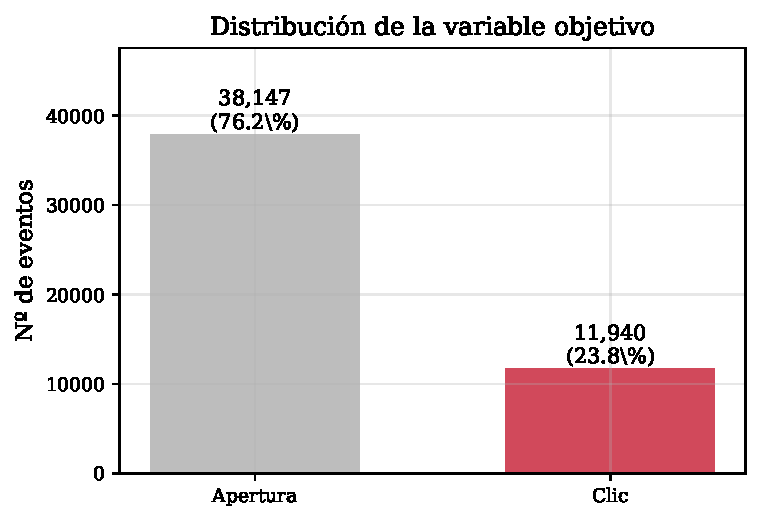
\includegraphics[width=0.55\textwidth]{fig_eda_target}
\caption{Distribution of the target variable in the training dataset: clicks versus opens.}
\label{fig:eda_target}
\end{figure}

\subsection{Resampling comparison}

The \emph{raw} dataset exhibits an extreme imbalance: of the 2.026.166 original events, only 2,2\,\% are clicks (1 click for every $\approx$44 non-clicks). So that the propensity model has enough positive examples, a \textbf{1:1 balanced sampling} is applied (all clicks plus an equal number of non-clicks) which, after deduplication and the filters, leaves the training set at 50.087 events with 23,8\,\% clicks (Figure~\ref{fig:eda_resampling}). The bias thus introduced is corrected a posteriori with the \textit{prior}-shift correction (Chapter~\ref{cap:propension}), which returns the probabilities to the real production scale.

\begin{figure}[htbp]
\centering
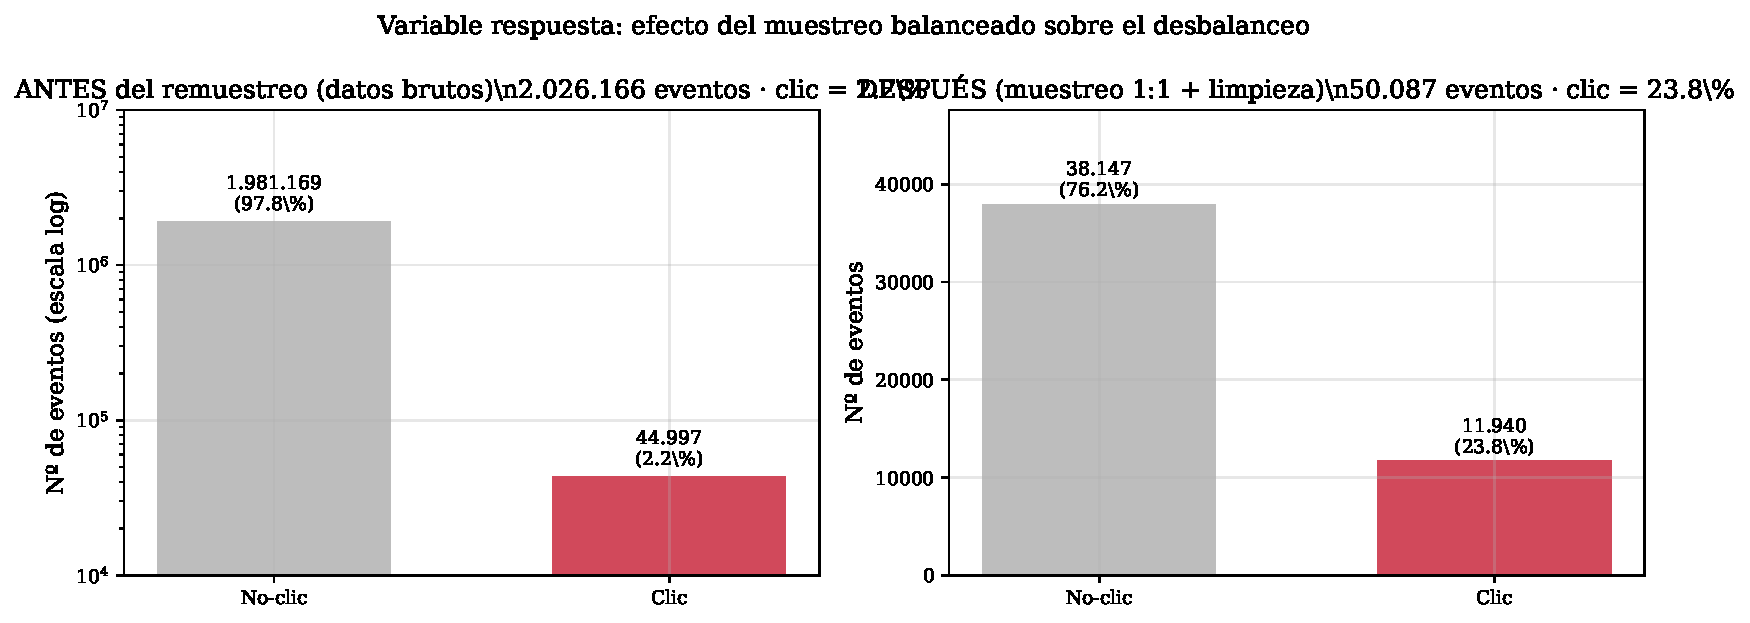
\includegraphics[width=\textwidth]{fig_eda_resampling}
\caption{Response variable \textbf{before} (raw data, logarithmic scale) and \textbf{after} balanced sampling and cleaning. The resampling raises the click prevalence from 2,2\,\% to 23,8\,\%, endowing the model with enough positive examples.}
\label{fig:eda_resampling}
\end{figure}

\paragraph{Effect on the observed variables.} Balanced sampling
changes the prevalence of the response without distorting the composition of the sample.
Table~\ref{tab:antes_despues} and Figure~\ref{fig:eda_antes_despues} compare, before and after, the
\emph{observed} variables (not the synthetic demographic ones, which are added later). The structure is
preserved: \textbf{age} is practically identical (mean 49,2 vs.\ 49,6; median 49) and the
sector mix is maintained (insurance dominates with $\approx$40--46\,\% in both; the order of the
main sectors does not change). The only appreciable shift is in \textbf{gender}: the proportion
of men rises from 43,5\,\% to 49,1\,\%, an expected effect because clicks tend to come from men
(their \textit{CTR} is somewhat higher) and the sampling retains all clicks; the resampling
thus rebalances the response without materially biasing the profile of the sample.

\begin{table}[htbp]
\centering
\caption{Descriptive statistics of the observed variables: before (raw) vs.\ after resampling}
\label{tab:antes_despues}
\begin{tabular}{lrrrrr}
\toprule
\textbf{Set} & \textbf{Events} & \textbf{Click \%} & \textbf{Users} & \textbf{Mean age} & \textbf{Men \%} \\
\midrule
Before (raw)        & 2.026.166 & 2,2  & 306.476 & 49,2 & 43,5 \\
After (balanced) & 50.087    & 23,8 & 35.405  & 49,6 & 49,1 \\
\bottomrule
\end{tabular}
\end{table}

\begin{figure}[htbp]
\centering
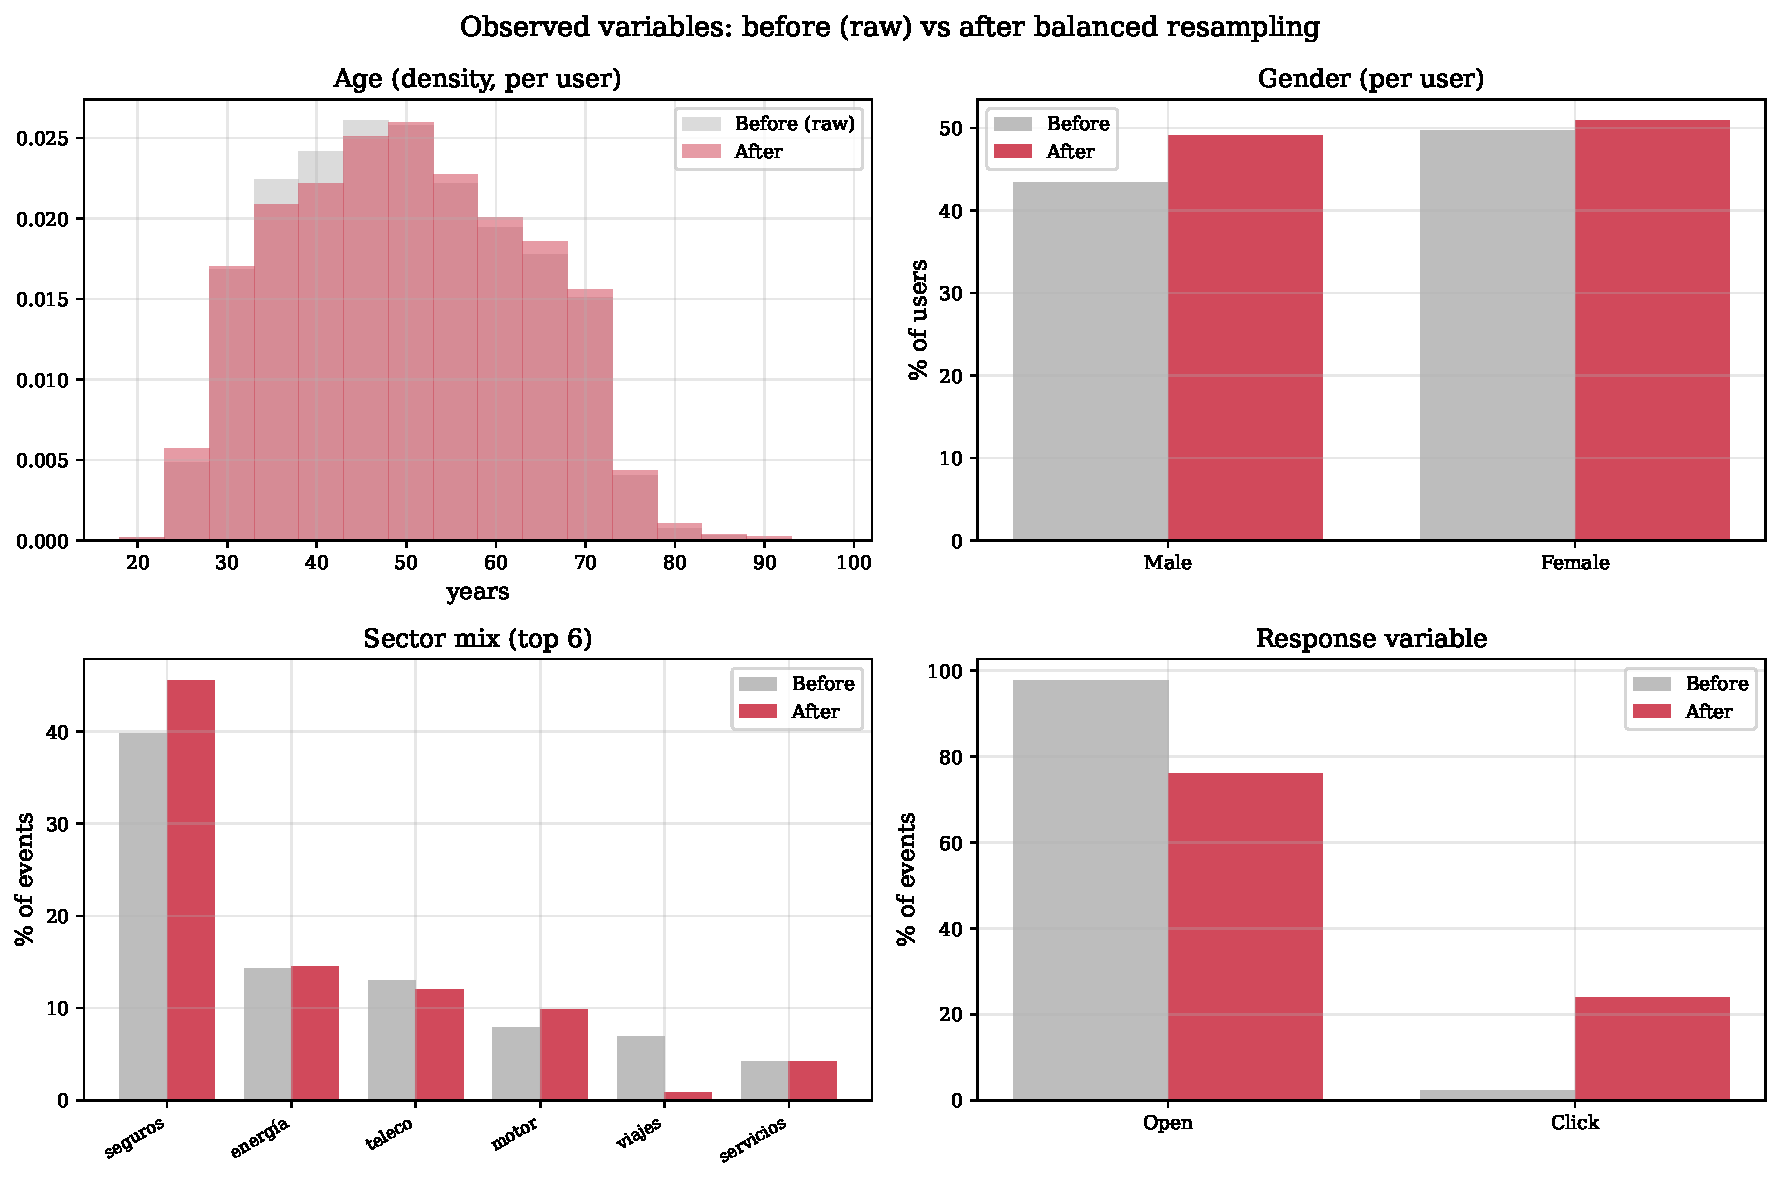
\includegraphics[width=\textwidth]{fig_eda_antes_despues}
\caption{Observed variables before (grey) vs.\ after (red) resampling: age and gender per user, sector mix and response variable. The resampling rebalances the response while preserving age and sector; gender shifts slightly towards men.}
\label{fig:eda_antes_despues}
\end{figure}

\subsection{Demographic profile of the users}

Figure~\ref{fig:eda_demographics} summarises the main user variables. \textbf{Age} is concentrated between 35 and 64 years (mean 50, range 20--117); for modelling it is discretised into six bands (\texttt{age\_cat}: 18-24, 25-34, 35-44, 45-54, 55-64 and 65+), with 45-54 being the most populated. \textbf{Gender} is practically balanced. \textbf{Employment status} reflects the INE rates (around 53\,\% employed), \textbf{marital status} predominates in ``married'' and the \textbf{income class} (purchasing power index, IPA) is concentrated in the medium and medium-low levels. Apart from age and the geographic variables, these attributes are synthetic imputations, with the quality caveat already noted (``Fundamental limitation'').

\begin{figure}[htbp]
\centering
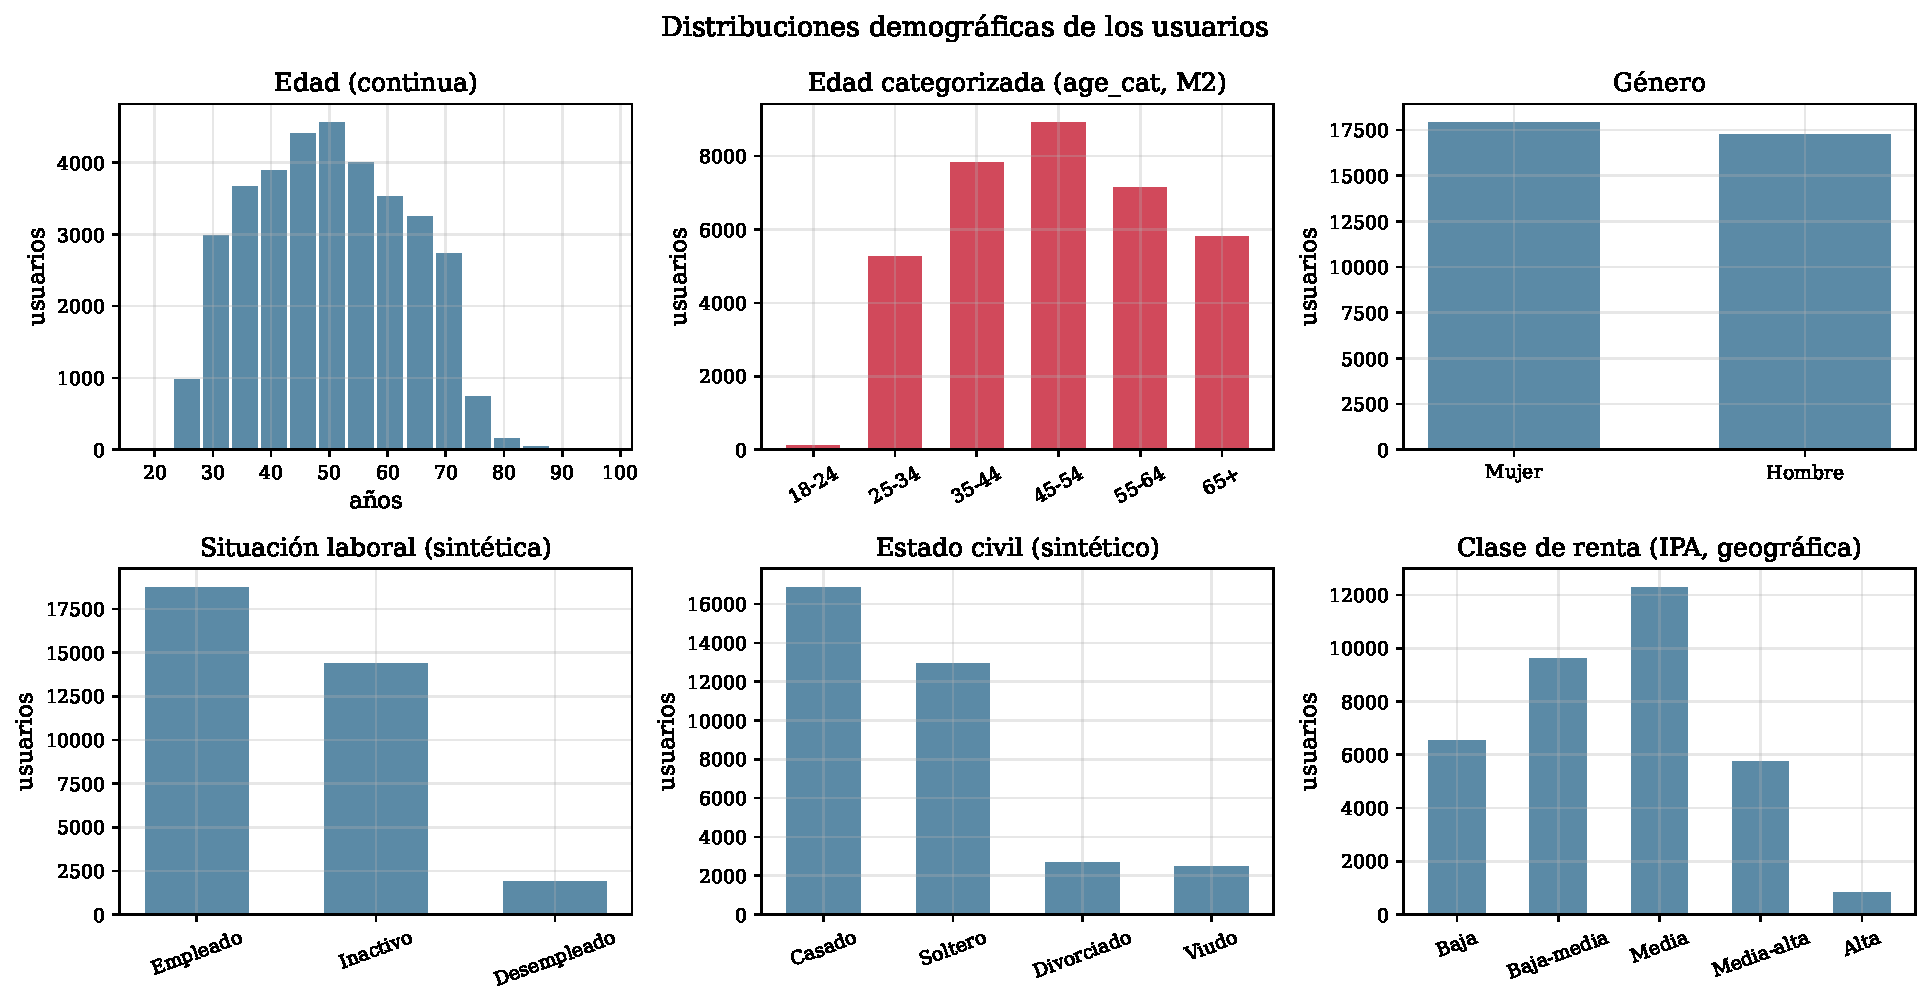
\includegraphics[width=0.92\textwidth]{fig_eda_demographics}
\caption{Demographic distributions of the users: age (continuous and categorised into the \texttt{age\_cat} bands of the M2 model), gender, employment status, marital status and income class (IPA).}
\label{fig:eda_demographics}
\end{figure}

\subsection{Behaviour by sector}

The click rate varies notably according to the \textbf{sector} of the product (Figure~\ref{fig:eda_ctr_sector}). \texttt{motor} is the sector with the highest propensity (0,37), followed by \texttt{servicios legales} (0,29) and \texttt{hogar} (0,27); \texttt{seguros}, the one with the largest volume, with 22.833 events, has a rate of 0,26, while \texttt{sorteos} (0,10) and \texttt{derechos humanos} (0,07) are the least effective. This heterogeneity between sectors suggested \emph{a priori} a hierarchical sector\,$\rightarrow$\,product architecture (first estimating the sector propensity and then refining the specific product). However, the comparison of the propensity module (Chapter~\ref{cap:propension}) shows that this decomposition worsens performance across all algorithms, so the sector is finally incorporated as one more variable of a flat model.

\begin{figure}[htbp]
\centering
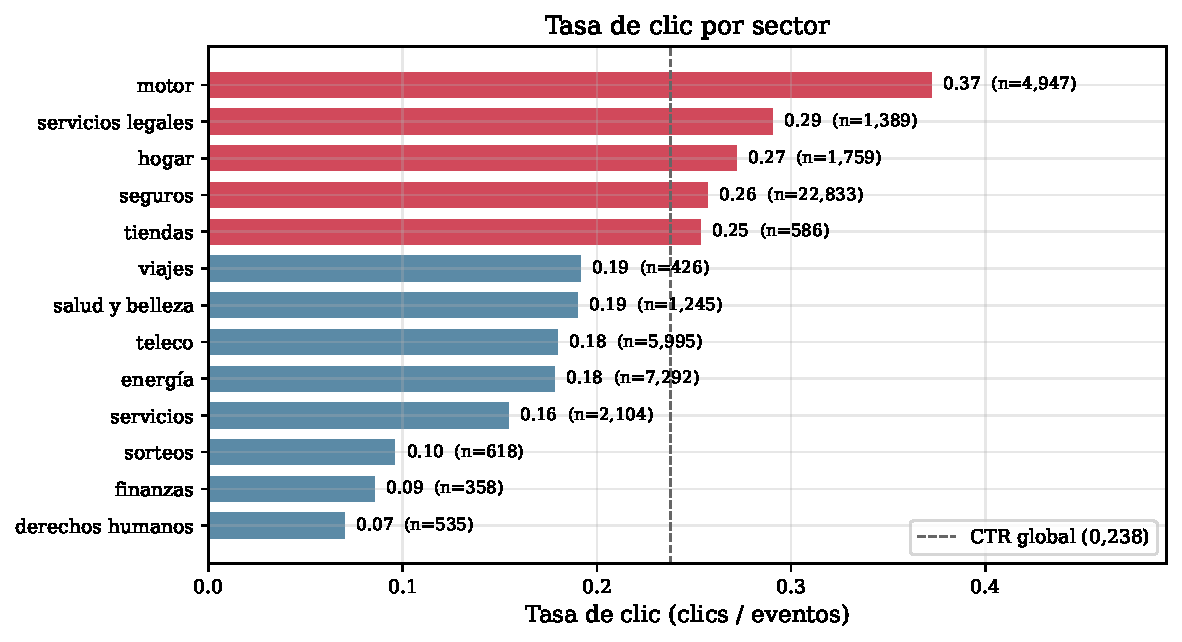
\includegraphics[width=0.85\textwidth]{fig_eda_ctr_sector}
\caption{Click rate by sector (only sectors with $\geq$100 events). The dashed line marks the overall rate (0,238); in red, the sectors above the mean.}
\label{fig:eda_ctr_sector}
\end{figure}

\subsection{Click rate by demographic variables}

The \emph{real} demographic variables (age and gender, the only observed and non-imputed ones) barely discriminate the click propensity (Figure~\ref{fig:eda_ctr_demo}). By \textbf{gender}, men click somewhat more than women (0,26 versus 0,22). By \textbf{age band}, the rate ranges between 0,20 (25--44 years) and 0,30 (55--64 years), with a gentle U-shaped pattern; the 18--24 band, with an apparently high rate (0,31), barely has 179 events and is not conclusive. The demographic differences in the click rate are modest (of the order of $\pm0{,}05$ around the mean of 0,238) compared with the strong variation by sector (from 0,07 to 0,37). This contrast anticipates the central finding of the propensity module (Chapter~\ref{cap:propension}): the signal resides much more in the \emph{product} than in the user's \emph{profile}.

\begin{figure}[htbp]
\centering
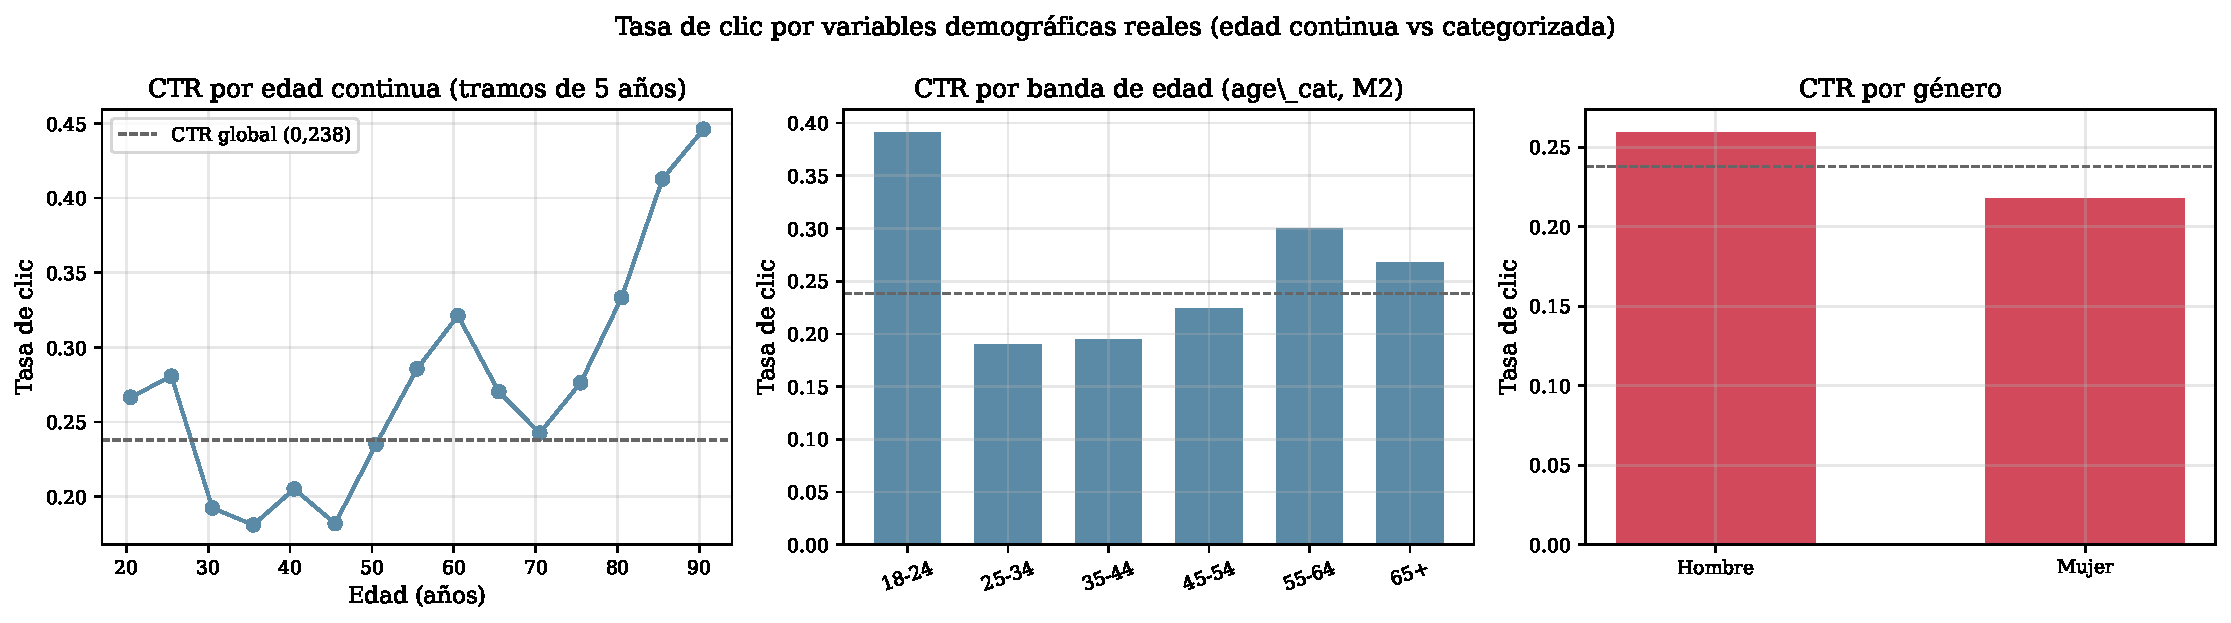
\includegraphics[width=0.92\textwidth]{fig_eda_ctr_demo}
\caption{Click rate by age band (left) and by gender (right). The dashed line marks the overall rate (0,238). The demographic differences are modest compared with those of the sector.}
\label{fig:eda_ctr_demo}
\end{figure}

\subsection{Product catalogue and cost per lead (CPL)}

The catalogue is concentrated: the 25 categories are not distributed uniformly. Figure~\ref{fig:eda_products} (left) shows the twelve categories with the most events; \texttt{health\_insurance} (10.623 events), \texttt{energy\_plan} and \texttt{funeral\_insurance} lead the volume. This concentration is relevant for the recommendation: the three most clicked categories account for 45\,\% of all clicks and the top five for 60\,\%, which turns \emph{popularity} into a \textit{baseline} that is hard to beat (Chapter~\ref{cap:recomendador}). The colour of each bar indicates whether its CTR exceeds the mean: categories such as \texttt{vehicle\_purchase} (CTR 0,43) or \texttt{home\_security} (0,33) are very effective despite their lower volume.

The \textbf{CPL} (cost per lead, interpreted as the profit that each click yields in the ROI analysis) is available for 54 of the 70 products; in the records with no CPL reported it is imputed with the median of 8\,\euro. Its distribution (Figure~\ref{fig:eda_products}, right) is asymmetric, with most products between 5 and 12\,\euro\ and a tail up to 31\,\euro; the sectors with the highest mean CPL are \emph{salud y belleza} (19\,\euro) and \emph{hogar} (14,5\,\euro). These figures feed the economic analysis of Chapter~\ref{cap:negocio}.

\begin{figure}[htbp]
\centering
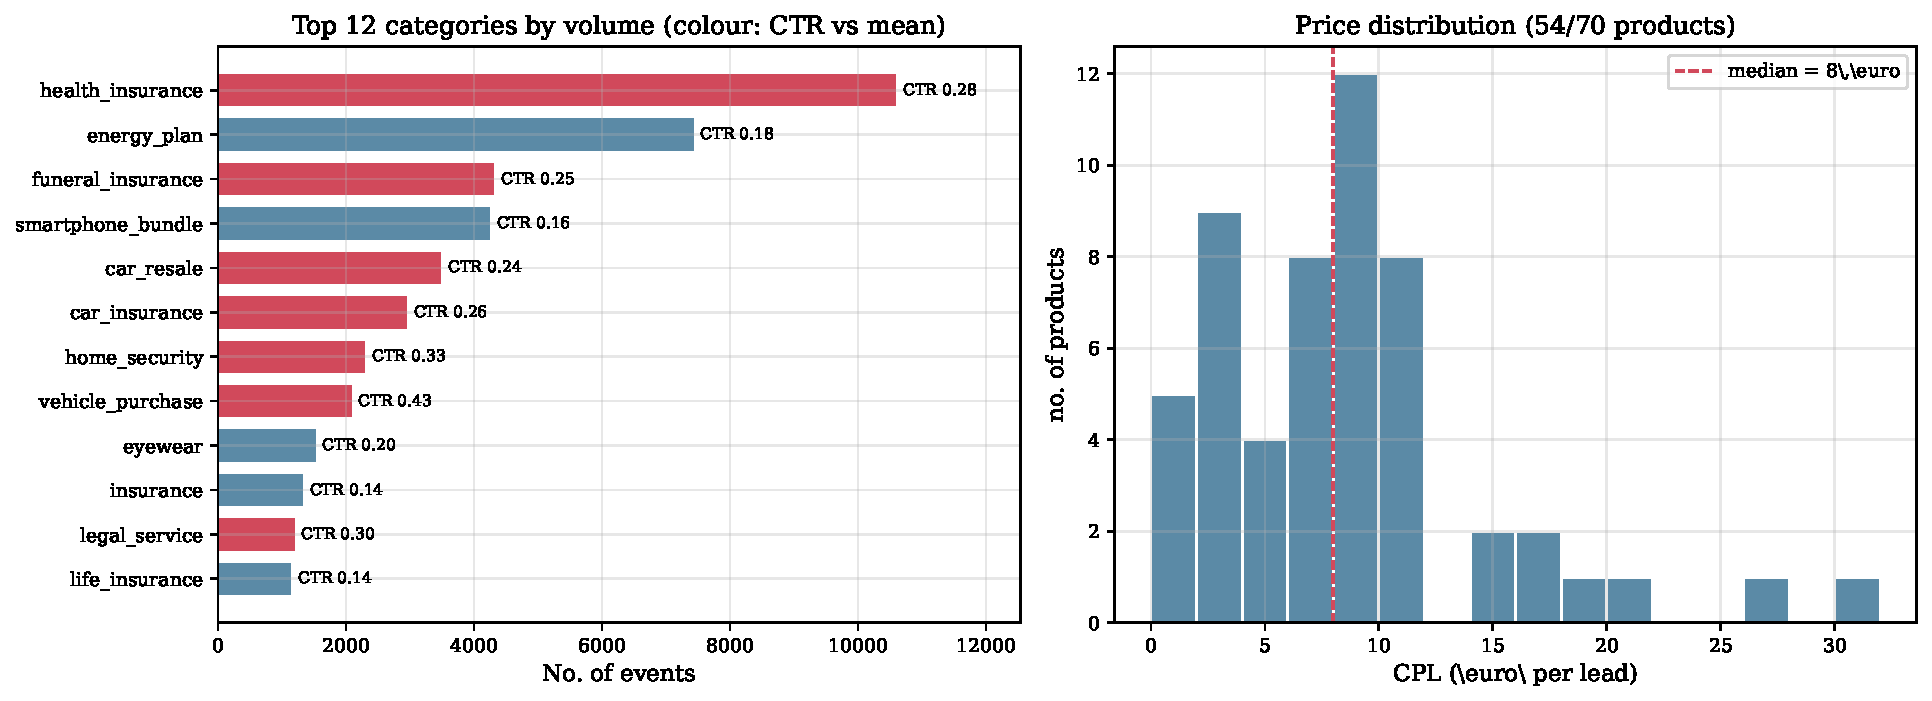
\includegraphics[width=\textwidth]{fig_eda_products}
\caption{Left: top 12 categories by event volume, coloured according to whether their CTR exceeds (red) or not (blue) the overall mean; the CTR of each one is annotated. Right: distribution of the CPL among the products that have it reported.}
\label{fig:eda_products}
\end{figure}

\subsection{Sparsity and activity per user}

The most important structural constraint of the project is the \textbf{scarcity of interactions per user} (Figure~\ref{fig:eda_sparsity}): 83,8\,\% of users have a single recorded event, the mean is 1,32 events and the maximum, 42. Combined with the 70 products, this produces a user--product matrix that is 98,1\,\% empty. The methodological consequence is direct: with so little individual history, classical collaborative filtering and a purely individual recommender are not viable, and approaches based on \emph{characteristics} (of the user and, above all, of the product) and on behavioural \emph{segments} are called for.

\begin{figure}[htbp]
\centering
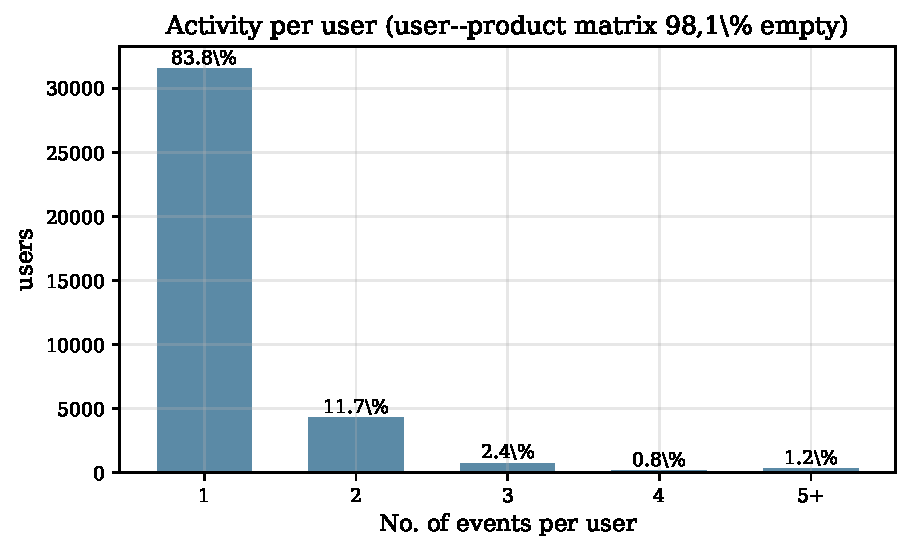
\includegraphics[width=0.6\textwidth]{fig_eda_sparsity}
\caption{Number of events per user (grouping users with five or more into ``5+''). The vast majority interact only once.}
\label{fig:eda_sparsity}
\end{figure}

\subsection{Temporal evolution}

Activity is not uniform over time (Figure~\ref{fig:timeseries}): after a gradual start, the volume of clicks is concentrated between August and December 2025, preceded by a period of low activity (fewer than 50 clicks per week) before 28 July 2025. This concentration conditions the temporal forecasting module (M4), which only has around 22 weeks of active history.

\begin{figure}[htbp]
\centering
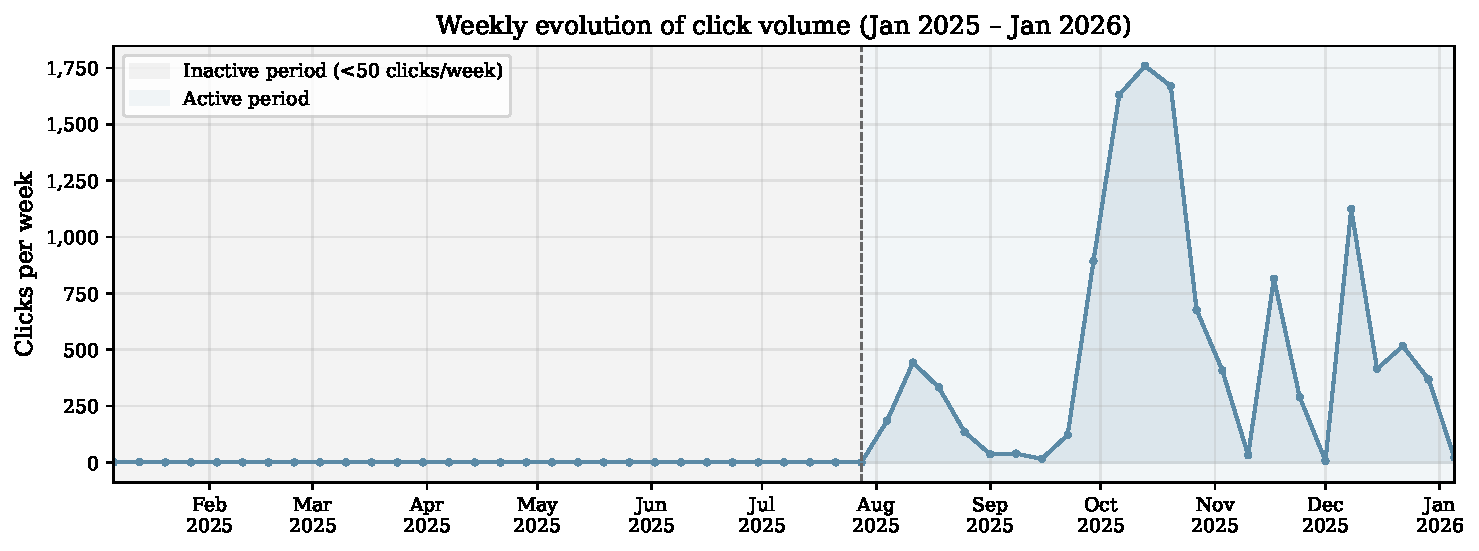
\includegraphics[width=\textwidth]{fig_timeseries}
\caption{Weekly evolution of the click volume (January 2025 -- January 2026). The grey shaded band delimits the inactive period prior to the start of the active campaign (28 July 2025).}
\label{fig:timeseries}
\end{figure}

\subsection{Data quality}

\paragraph{Cleaning funnel.} The final dataset is the result of a chain of successive filters over the raw data, summarised in Table~\ref{tab:funnel}. Each step responds to an explicit quality criterion (removing records without key information, safeguarding privacy, avoiding duplicates and ensuring a resolvable geographic profile). The most relevant drop in users occurs when requiring a postal code\,$\rightarrow$\,municipality correspondence (6,4\,\% not resolvable), discarded so as not to introduce arbitrarily imputed geographic profiles.

\begin{table}[htbp]
\centering
\caption{Cleaning funnel: from the raw data to the final modelling dataset}
\label{tab:funnel}
\begin{tabular}{p{6.2cm}rrr}
\toprule
\textbf{Stage} & \textbf{Events} & \textbf{Clicks} & \textbf{Users} \\
\midrule
Raw data (all raw files)                             & 2.026.166 & 44.997 (2,2\,\%) & --- \\
1:1 balanced sample + cleaning (dedup email/subject, age 18--120, missing) & 50.087 & 11.940 (23,8\,\%) & 37.815 \\
After requiring postal code\,$\rightarrow$\,municipality resolution    & 50.087 & 11.940 & 35.405 \\
\bottomrule
\end{tabular}
\end{table}

\paragraph{Completeness and consistency.} After cleaning, the tables present no missing values in the variables used by the models (the only unpopulated column is \texttt{district\_name}, not used in modelling); the CPL, absent in part of the records, is imputed with the median (8\,\euro) only for the ROI analysis. No duplicates were detected in the dimensional tables after the event deduplication. The coverage of the geographic enrichment reaches 100\,\% of the 35.405 final users. The main quality caveat is the one already noted: the \emph{fine-grained} demographic variables (employment, household, vehicle, etc.) are ecological imputations whose individual quality is bounded by construction (``Fundamental limitation'').

\chapter{Diseño del sistema y marco de evaluación}
\label{cap:evaluacion}

Este capítulo presenta una visión general del pipeline y, sobre todo, el marco de evaluación común a todos los módulos: qué métricas se usan y cómo interpretarlas, cómo se valida sin fuga de datos y qué pruebas estadísticas respaldan cada comparación. Reunir estas definiciones aquí evita repetirlas en cada módulo y permite que los capítulos siguientes se centren en sus resultados.

\section{Visión general del pipeline}

El sistema se organiza en un pipeline secuencial que transforma los datos brutos de campaña en predicciones y recomendaciones accionables, agrupado en cuatro bloques funcionales:
\begin{itemize}
    \item \emph{Bloque I — Preparación de datos} (\texttt{01\_clean}, \texttt{02\_geo}, \texttt{03\_users}): limpieza, construcción de tablas dimensionales y enriquecimiento demográfico (Capítulo~\ref{cap:datos}).
    \item \emph{Bloque II — Segmentación} (\texttt{05\_demo\_segmentation}, \texttt{06\_segmentation}): dos niveles de agrupación de usuarios, M0 (demográfica) y M1 (comportamental) (Capítulo~\ref{cap:segmentacion}).
    \item \emph{Bloque III — Modelado predictivo} (\texttt{07\_propensity}, \texttt{08\_recommender}): propensión al clic (M2, Capítulo~\ref{cap:propension}) y recomendador por cluster (M3, Capítulo~\ref{cap:recomendador}).
    \item \emph{Bloque IV — Previsión temporal} (\texttt{09\_forecast}): predicción del volumen semanal de clics (M4, Capítulo~\ref{cap:forecast}).
\end{itemize}
Como análisis complementarios se incluyen un diagnóstico de estabilidad del número de clusters (\texttt{05b\_k\_stability}), un modelo inverso producto\,$\rightarrow$\,perfil (\texttt{10\_inverse\_profile}) y un ejemplo de despliegue con análisis de retorno (Capítulo~\ref{cap:negocio}). Cada capítulo de módulo presenta de forma conjunta su \emph{método} y sus \emph{resultados}, para facilitar la lectura.

\section{Métricas de evaluación}
\label{sec:metricas}

Cada tipo de problema exige métricas distintas. A continuación se definen las empleadas y, lo más importante, cómo interpretarlas: qué valor es bueno y cuál es el de referencia o ``azar''.

\subsection{Propensión al clic (clasificación binaria)}

El problema es de clases desbalanceadas (pocos clics frente a muchas no-interacciones), lo que condiciona la elección de métricas: la \emph{exactitud} (\textit{accuracy}) engaña, porque un modelo que prediga ``nunca clic'' acertaría la mayoría de las veces sin ser útil.

\begin{itemize}
    \item \textbf{PR-AUC} (área bajo la curva \textit{precision-recall}), métrica principal. Resume cómo de bien el modelo identifica la clase rara (el clic) a distintos umbrales. Va de 0 a 1; mayor es mejor. Su valor de \emph{referencia} (lo que daría el azar) no es 0,5 sino la prevalencia de positivos: aquí $\approx0{,}238$. Por eso un PR-AUC de 0,40 sobre una prevalencia de 0,24 sí indica señal real. Se prefiere a la AUC-ROC en desbalanceo porque se centra en la clase positiva~\cite{davisgoadrich2006,saito2015}.
    \item \textbf{AUC-ROC} (área bajo la curva ROC)~\cite{fawcett2006}, métrica de apoyo. Mide la capacidad de \emph{ordenar} un positivo por encima de un negativo elegidos al azar. Va de 0 a 1: 0,5 es azar, 1 es perfecto. Orientativamente, $\approx0{,}7$ es modesto, $0{,}8$ bueno y $\geq0{,}9$ excelente. En desbalanceo tiende a ser \emph{optimista}, de ahí que la principal sea PR-AUC.
    \item \textbf{Brier score}~\cite{brier1950}, calidad de la \emph{calibración}. Mide si las probabilidades son \emph{realistas} (no solo si el orden es correcto): es el error cuadrático medio entre la probabilidad predicha y el resultado real (0/1). Menor es mejor (0 = perfecto).
    \item \textbf{F1, MCC y \textit{Balanced Accuracy}}, calidad de la decisión binaria a un umbral fijo (aquí, la prevalencia 0,238). El F1 es la media armónica de precisión y exhaustividad (0 a 1). El MCC (coeficiente de correlación de Matthews~\cite{matthews1975}) resume la matriz de confusión completa y es robusto al desbalanceo: va de $-1$ a $1$, con 0 = azar. La \textit{Balanced Accuracy} promedia el acierto en cada clase por separado (0,5 = azar).
\end{itemize}

\subsection{Recomendación (calidad del \textit{ranking})}

Aquí no se predice un número, sino un \emph{orden} de categorías; las métricas miden si las categorías relevantes para el usuario aparecen arriba en una lista de tamaño $K$.
\begin{itemize}
    \item \textbf{Hit Rate@$K$} (HR@$K$): fracción de usuarios para los que \emph{al menos una} categoría relevante está entre las $K$ recomendadas. Responde ``¿acerté algo en el top-$K$?''. Va de 0 a 1.
    \item \textbf{NDCG@$K$} (\textit{Normalized Discounted Cumulative Gain})~\cite{jarvelin2002}: como HR pero premia el orden, dando más peso a los aciertos en las primeras posiciones. De 0 a 1.
    \item MAP@$K$ (\textit{Mean Average Precision}): precisión media a lo largo de la lista, también sensible al orden. De 0 a 1.
\end{itemize}

\subsection{Previsión temporal}

Para el volumen semanal de clics se usan métricas de error de predicción (menor es mejor):
\begin{itemize}
    \item \textbf{MAE} (error absoluto medio) y \textbf{RMSE} (raíz del error cuadrático medio): en las mismas unidades que la serie (clics/semana); el RMSE penaliza más los errores grandes.
    \item MAPE (error porcentual absoluto medio): el error relativo en \%; cómodo de interpretar pero inestable cuando los valores reales son pequeños.
\end{itemize}

\section{Validación sin fuga de datos}
\label{sec:validacion}

La estimación fiable del rendimiento exige evitar la \emph{fuga de datos} (\textit{data leakage}): que el modelo acceda en entrenamiento a información que no tendría en producción, lo que infla artificialmente las métricas~\cite{kaufman2012leakage}. Se emplean tres esquemas según el módulo:
\begin{itemize}
    \item \emph{Validación cruzada agrupada por usuario} (\texttt{GroupKFold}, M2): reparte los datos en 5 \emph{folds} garantizando que ningún usuario esté a la vez en entrenamiento y validación. Es imprescindible aquí porque las variables de un usuario son idénticas en todos sus eventos; sin agrupar, el modelo ``memorizaría'' al usuario y sobreestimaría su capacidad. Mide la generalización a usuarios \emph{nuevos}.
    \item \emph{Validación cruzada temporal} (\texttt{TimeSeriesSplit}, modelo \textit{warm} y M4): el entrenamiento es siempre \emph{pasado} y la validación \emph{futuro}, respetando el orden cronológico.
    \item \emph{Reconstrucción solo con \textit{train}} (M3): el segmento de cada usuario se recalcula usando únicamente los datos de entrenamiento, para que no ``conozca'' el periodo de test.
\end{itemize}

\paragraph{Corrección de prior (\textit{prior shift}).} El modelo de propensión se entrena con una muestra \emph{balanceada} (\textasciitilde24\,\% de clics) pero en producción la tasa real es $\approx 2$\,\%; sin ajuste, las probabilidades saldrían infladas. La transformación de Dal Pozzolo et al.~\cite{dalpozzolo2015} (ecuación~\ref{eq:prior_correction}) las reescala al prior real. Es monótona: cambia la magnitud de las probabilidades pero \emph{no} su orden, por lo que no afecta a las métricas de \textit{ranking} (PR-AUC, AUC-ROC).

\paragraph{Validación cruzada frente a \textit{bootstrap}.} Son complementarios y responden a preguntas distintas. La validación cruzada mide \emph{cómo de bien generaliza} el modelo (reentrena $k$ veces, cada dato es test una vez). El \textit{bootstrap} mide la \emph{incertidumbre} de una métrica ya calculada: remuestrea el conjunto de test al azar muchas veces (con reemplazo) y observa cuánto varía la métrica, lo que da un intervalo de confianza sin necesidad de reentrenar.

\section{Contraste estadístico}
\label{sec:tests}

Que un modelo obtenga una métrica algo mejor que otro \emph{no} basta para afirmar que es superior: la diferencia podría deberse al azar de la muestra concreta. Las pruebas estadísticas cuantifican esa duda. La idea común es el \emph{$p$-valor}: la probabilidad de observar una diferencia tan grande como la medida \emph{si en realidad no hubiera diferencia}; un $p<0{,}05$ se interpreta como evidencia de que la diferencia no es casualidad. El uso de pruebas no paramétricas para comparar modelos sigue las recomendaciones de Dem\v{s}ar~\cite{demsar2006}. Las pruebas empleadas son:

\begin{itemize}
    \item \textbf{Intervalo de confianza \textit{bootstrap}}~\cite{efron1979}: se remuestrea el test con reemplazo (1.000 veces) y se recalcula la métrica o su diferencia. Si el intervalo al 95\,\% de una diferencia \emph{no incluye el 0}, la diferencia es robusta. No depende del número de \emph{folds}.
    \item \textbf{Test de Wilcoxon (pareado)}~\cite{wilcoxon1945}: compara dos modelos \emph{fold a fold}, sin asumir normalidad. \emph{Limitación} importante: con 5 \emph{folds} el menor $p$-valor posible es 0,0625, así que un resultado no significativo puede deberse a falta de potencia, no de diferencia; por eso se apoya en el \textit{bootstrap}.
    \item \textbf{Test de Friedman}~\cite{friedman1937}: prueba \emph{global} para comparar tres o más métodos sobre los mismos sujetos (``¿hay alguna diferencia entre ellos?''). Se hace antes de comparar pares.
    \item \textbf{Test de McNemar}~\cite{mcnemar1947}: compara dos métodos \emph{caso a caso} en acierto/fallo, fijándose solo en los casos en que discrepan. Útil para contrastar la tasa de acierto (HR@5) entre el recomendador y un \textit{baseline}.
    \item \textbf{Corrección de Holm}~\cite{holm1979}: al realizar \emph{varias} comparaciones a la vez, la probabilidad de un falso positivo se acumula. Holm endurece el umbral de significación de forma secuencial (al $p$ más pequeño le exige el listón más estricto), controlando ese riesgo.
    \item \textbf{Test de Diebold-Mariano (DM)}~\cite{diebold1995}: el equivalente para comparar \emph{predicciones de series temporales}; contrasta los errores semana a semana de dos modelos de \textit{forecast}. Con muestras pequeñas se aplica la corrección de Harvey-Leybourne-Newbold~\cite{harvey1997} (factor de muestra reducida y $t$ de Student), imprescindible aquí por disponer de pocos orígenes.
    \item \emph{Tamaños de efecto}: el $p$-valor dice si una diferencia existe, no \emph{cómo de grande} es. Se reportan la W de Kendall (para el Friedman; 0 = sin efecto, 1 = efecto máximo) y la correlación rango-biserial $|r|$ (para los Wilcoxon pareados; orientativamente, $0{,}1$ pequeño, $0{,}3$ medio, $0{,}5$ grande).
\end{itemize}

Todas las semillas aleatorias se fijan en 42 para garantizar la reproducibilidad (Apéndice~\ref{ap:reproducibilidad}).


\part{Models}
\chapter{Módulo M0/M1 — Segmentación de clientes}
\label{cap:segmentacion}

Este capítulo agrupa los dos niveles de segmentación no supervisada de usuarios, presentando para cada uno su método y sus resultados. La segmentación \textbf{demográfica} (M0) asigna un perfil a usuarios nuevos sin historial; la \textbf{comportamental} (M1) agrupa a los usuarios activos por su patrón de interacción.

\section{M0 — Segmentación demográfica (arranque en frío)}

\subsection{Método}

La segmentación demográfica tiene como objetivo asignar un perfil de comportamiento esperado a usuarios nuevos para los que no existe historial de interacciones (\textit{cold start}). Se aplica sobre los 35.405 usuarios del dataset a partir de diez variables de perfil: edad \emph{categorizada} en bandas (\texttt{age\_cat}, las mismas que en M2), género, situación laboral, estado civil, tenencia de vehículo, tamaño del hogar, número de habitaciones, índice de poder adquisitivo (IPA), tipo de municipio y distancia al núcleo urbano más próximo. Las variables categóricas se codificaron ordinalmente de acuerdo con su significado semántico antes de aplicar el escalado estándar.

\paragraph{Selección del espacio de \textit{embedding}.} Se compararon tres espacios de representación para el clustering posterior mediante el coeficiente de silueta con $k=2$ y $n=5.000$ muestras: (1) el espacio original estandarizado (10 dimensiones); (2) una reducción por PCA hasta explicar el 80\,\% de la varianza (8 componentes); y (3) un \textit{embedding} no lineal mediante autoencoder (4 dimensiones latentes). El autoencoder tiene la arquitectura:
\[
10 \xrightarrow{\text{Dense}(64)} \xrightarrow{\text{BN}} \xrightarrow{\text{Dense}(32)} \xrightarrow{\text{Dense}(4)} \xrightarrow{\text{Dense}(32)} \xrightarrow{\text{BN}} \xrightarrow{\text{Dense}(64)} \xrightarrow{\text{Dense}(10)}
\]
(donde BN denota \textit{batch normalization}) y entrenado con pérdida MSE, optimizador Adam, \textit{batch size} 256, \textit{validation split} 0,1 y parada temprana (paciencia 10 épocas). El autoencoder obtuvo la mayor silueta y fue seleccionado como espacio de clustering (resultados abajo). Se eligió frente a PCA por su capacidad de capturar relaciones \emph{no lineales} entre las variables de perfil, que una reducción lineal no recoge~\cite{hinton2006}. No obstante, conviene matizar que, dado que el espacio demográfico resulta prácticamente un continuo (como muestra más adelante el diagnóstico de estabilidad de $k$), \textbf{PCA habría sido una alternativa más simple y de resultados comparables}; el autoencoder aporta una mejora modesta de cohesión a cambio de mayor complejidad.

Conviene aclarar por qué la silueta sí sirve aquí para elegir el \emph{espacio} pero no para elegir el \emph{número de clusters}: para comparar espacios se fija un mismo $k=2$ y se mide cuál separa mejor con ese $k$ común (una comparación \emph{relativa} y justa); en cambio, al barrer $k$ la silueta crece de forma monótona y su máximo no señala un número natural de grupos, por lo que para esa segunda decisión se recurre a la estabilidad (ARI).

\paragraph{Selección de $k$.} Se evaluaron KMeans para $k \in \{2,\ldots,12\}$ con cuatro métricas: silueta y Calinski-Harabasz (maximizar), Davies-Bouldin (minimizar) e inercia (codo). Como se verá, la silueta y el Calinski-Harabasz crecen de forma \emph{monótona} con $k$ (sin máximo interior), lo que indica que el espacio demográfico es prácticamente un continuo sin un número natural de grupos. Por ello la elección de $k$ se basó en la \textbf{estabilidad} de las asignaciones mediante un diagnóstico por re-muestreo (\textit{Adjusted Rand Index}, ARI~\cite{hubert1985}). Como referencia se ejecutó también HDBSCAN (búsqueda de \texttt{min\_cluster\_size}); su mejor configuración produjo 18 clusters con un 5,5\,\% de usuarios sin asignar (ruido). Se seleccionó KMeans por su \textbf{cobertura total} (0\,\% de ruido) y un número de grupos más manejable.

\subsection{Resultados}

El espacio del autoencoder (4 dimensiones latentes) superó al PCA y al original en cohesión de clustering medida por silueta (0,344 frente a 0,142 y 0,129 en $k=2$). Se seleccionó KMeans con $k=10$ sobre dicho espacio. Los 10 clusters presentan diferencias interpretables: el de mayor tamaño ($n\approx4.900$; 13,8\,\%) agrupa al perfil modal, mientras que los minoritarios ($n\approx1.500$) recogen perfiles de grandes viviendas o de municipios pequeños. La Figura~\ref{fig:umap_m0} muestra la proyección UMAP de los clusters.

\begin{figure}[htbp]
\centering
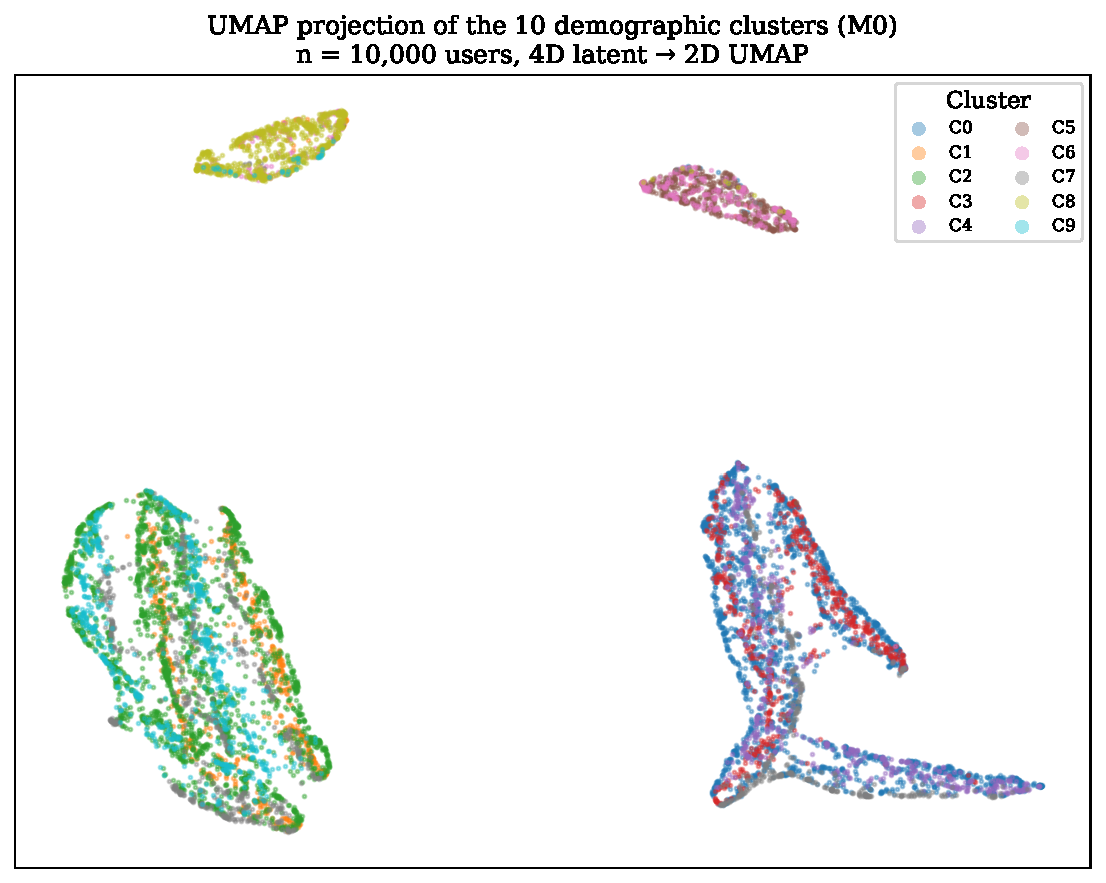
\includegraphics[width=0.80\textwidth]{fig_umap_m0}
\caption{Proyección UMAP bidimensional del espacio latente de 4 dimensiones del autoencoder (M0). Cada punto es un usuario coloreado por su cluster demográfico ($k=10$).}
\label{fig:umap_m0}
\end{figure}

\paragraph{Diagnóstico de estabilidad de $k$.} Las métricas puntuales no fijan un $k$ óptimo: la silueta crece de forma monótona con $k$ (de 0,35 en $k=2$ a 0,46 en $k=12$), señal de que el espacio demográfico es prácticamente un \emph{continuo} sin grupos naturales bien separados; su máximo coincide con el tope del rango de búsqueda y no es un criterio fiable. Para decidir con rigor se evaluó la \textbf{estabilidad} del clustering repitiendo KMeans 15 veces sobre submuestras del 80\,\% y midiendo el ARI entre re-muestreos, que cuantifica cuán consistentes son las asignaciones. La Figura~\ref{fig:kstability} resume el barrido. El ARI se mantiene \textbf{muy alto en todo el rango} ($0{,}96$--$1{,}0$): el clustering es estable para casi cualquier $k$, de modo que la estabilidad por sí sola no señala un único valor ($k=10$ obtiene ARI $0{,}984$, muy próximo al máximo, que está en $k=11$ con $0{,}998$). \textbf{Se adopta $k=10$}: dentro de esa meseta de alta estabilidad es un valor que combina buena cohesión (silueta $\approx0{,}43$), una granularidad interpretable y coherencia con el resto del \textit{pipeline}. Este valor se propaga a los módulos dependientes (propensión M2, arranque en frío de M3 y modelo inverso).

\begin{figure}[htbp]
\centering
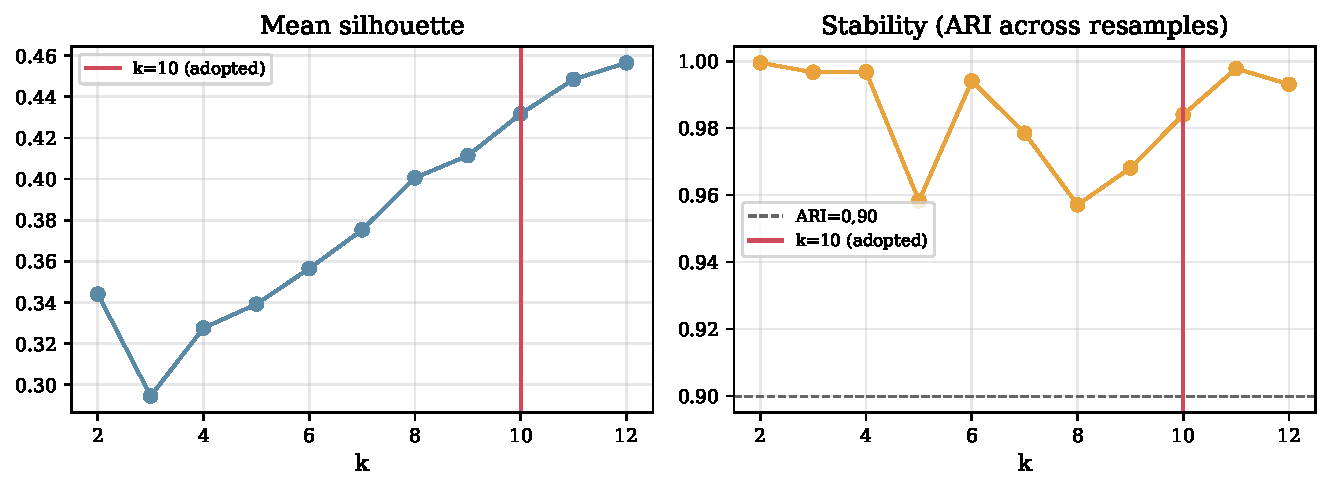
\includegraphics[width=\textwidth]{fig_k_stability}
\caption{Estabilidad del clustering demográfico frente al número de clusters $k$. Izquierda: silueta media por submuestreo. Derecha: ARI entre pares de re-muestreos (1 = clustering idéntico). Se marca $k=10$ (adoptado). El ARI es alto en todo el rango ($0{,}96$--$1{,}0$), por lo que la estabilidad no señala un único $k$ y se elige $k=10$ por cohesión, granularidad y coherencia del \textit{pipeline}.}
\label{fig:kstability}
\end{figure}

\section{M1 — Segmentación comportamental}

\subsection{Método}

La segmentación comportamental (M1) aplica el mismo marco sobre un espacio de características que combina el historial de interacciones con los atributos de usuario. Se construyen 46 variables en tres bloques:
\begin{itemize}
    \item \textbf{Actividad} (7 variables): número de eventos, clics, aperturas, productos, sectores, recencia y tasa de clic. Las variables de conteo se transforman con $\log(1+x)$ para reducir el sesgo de la distribución.
    \item \textbf{Sector} (18 variables): frecuencia de eventos y tasa de clic por sector (9 sectores).
    \item \textbf{Producto} (21 variables): frecuencia de eventos por categoría de producto (top 20 + \textit{other}).
\end{itemize}
La reducción dimensional se realizó con PCA fijando 26 componentes (varianza explicada $\geq 90$\,\%). Sobre el espacio PCA se evaluaron KMeans ($k \in \{4,\ldots,12\}$), GMM ($k \in \{3,\ldots,9\}$) y HDBSCAN, con el requisito adicional de que ningún cluster supere el 60\,\% de la base.

\subsection{Resultados}

KMeans con $k=12$ fue seleccionado (silueta 0,347) frente a GMM ($k=9$, silueta 0,249) y HDBSCAN (0,210; excluido por 46\,\% de \textit{outliers}). La distribución de los segmentos refleja la asimetría del dataset: el segmento 3 agrupa al 39,1\,\% de los usuarios ($n=13.858$) con \textit{click rate} de 0,01 (una única apertura sin clic en seguros); en el extremo opuesto, los segmentos 1 y 2 concentran usuarios de alta actividad (\textit{click rates} 0,95 y 0,99) pero solo el 8,3\,\% de la base. Esta segmentación es la que emplea el recomendador (Capítulo~\ref{cap:recomendador}).

\chapter{Módulo M2 — Modelo de propensión}
\label{cap:propension}

Este capítulo desarrolla el modelo de propensión al clic: primero su método (definición, muestreo, arquitectura, algoritmo y validación) y después sus resultados (corrección de una fuga, aportación de las variables, comparación de algoritmos, calibración, modelo \textit{warm} y estudios de ablación). La métrica principal es PR-AUC, adecuada ante el fuerte desbalanceo de clases (prevalencia $\approx0{,}238$); su interpretación y la de los tests se detallan en el Capítulo~\ref{cap:evaluacion}.

\section{Método}

\subsection{Definición del problema y variable objetivo}

El objetivo de M2 es estimar la propensión al clic de un par (usuario, producto): un \textit{score} con el que ordenar, para cada usuario, qué productos tienen más probabilidad de recibir un clic. La variable objetivo binaria es 1 si el evento registrado en \texttt{events.csv} es un clic y 0 si es una apertura. Más adelante se comparan dos formas de estimar ese \textit{score} (un modelo \emph{plano} y uno \emph{jerárquico} sector\,$\rightarrow$\,producto) y se justifica, con la evidencia empírica, por qué se adopta el plano.

\subsection{Estrategia de muestreo y corrección de prior}

El dataset de eventos presenta un click rate real de $\rho_\text{real} \approx 2\%$ en el dataset completo y de $\rho_\text{train} = 23{,}84\%$ en el sample procesado (resultado de la deduplicación y el muestreo balanceado descrito en el Capítulo~\ref{cap:datos}). Para permitir que el modelo aprenda la frontera de decisión con suficientes ejemplos positivos, se entrenó sobre el dataset balanceado. Las probabilidades predichas se corrigen a posteriori aplicando la transformación de la ecuación~\ref{eq:prior_correction} con $\rho_\text{real}=0{,}02$ y $\rho_\text{train}=0{,}2384$ (Sección~\ref{sec:validacion}).

\subsection{Arquitectura del modelo}

Las variables de \emph{producto} se incluyen porque el clic es una propiedad del \emph{par} (usuario, producto), no del usuario aislado: un único modelo alimentado solo con atributos de usuario devolvería el mismo valor para todos los productos de ese usuario y, por tanto, no podría ordenarlos. Para discriminar entre productos existen dos opciones: entrenar un modelo independiente por categoría (donde la identidad del producto queda implícita en \emph{qué} modelo se consulta) o emplear un único modelo que reciba el producto como variable de entrada. Esta segunda opción, además de no fragmentar los datos en muchos modelos pequeños, puede aprovechar los atributos del producto (en particular el texto del asunto) y generalizar a productos sin historial. Por eso se comparan la \textbf{Variante A} (un modelo por categoría con \emph{solo} variables de usuario, el enfoque demográfico tradicional) y la \textbf{Variante B} (un único modelo que añade variables de producto); la comparación de la Sección~\ref{sec:m2-variables} confirma que añadir variables de producto aporta de forma significativa.

Sobre esa base se evalúan además dos arquitecturas. La primera es un \textbf{modelo plano}: un único modelo estima directamente $P(\text{click}\mid u,\text{producto})$ y su salida se usa como \textit{score} para rankear los productos de cada usuario. La segunda es un \textbf{modelo jerárquico} en dos niveles inspirado en la decisión de compra: un Nivel 1 estima la propensión de sector $P(\text{click}\mid u,\text{sector})$, un Nivel 2 la condicional de producto $P(\text{click}\mid u,\text{sector},\text{producto})$ y el \textit{score} final es el producto de ambos, $p_\text{sector}\cdot p_\text{producto}$. La comparación de ambas arquitecturas (Sección~\ref{sec:m2-algos}) muestra que el modelo plano supera al jerárquico en \emph{todos} los algoritmos: la PR-AUC cae entre 0,014 y 0,028 al pasar a la variante jerárquica, y la multiplicación de las dos probabilidades, además de no aportar señal, descalibra las predicciones (el \textit{Brier} empeora de $\approx0{,}17$ a $\approx0{,}21$). La razón es que encadenar dos estimaciones imperfectas acumula su error en lugar de cancelarlo, y un único modelo plano ya puede usar el sector como una variable más sin pagar ese coste. Por eso se adopta el modelo plano. La estructura jerárquica se conserva como variante interpretable (descompone la decisión en sector y producto), pero no se adopta como modelo final.

\subsection{Algoritmo y características}

El algoritmo seleccionado es \textbf{LightGBM} \cite{ke2017lightgbm}, elegido tras comparar también una red neuronal (perceptrón multicapa), HistGradientBoosting, Random Forest y regresión logística sobre las mismas particiones; la comparación detallada (Sección~\ref{sec:m2-algos}) muestra diferencias pequeñas entre los métodos basados en árboles (con LightGBM y Random Forest a la cabeza y la red neuronal en último lugar), lo que confirma que el techo de rendimiento lo marcan los datos, no el algoritmo. Los hiperparámetros se recogen en la Tabla~\ref{tab:lgbm_params}; \texttt{num\_leaves} se redujo a 15 porque, con señal débil, un modelo más regularizado generaliza mejor.

\begin{table}[htbp]
\centering
\caption{Hiperparámetros del modelo LightGBM (M2)}
\label{tab:lgbm_params}
\begin{tabular}{ll}
\toprule
\textbf{Parámetro} & \textbf{Valor} \\
\midrule
\texttt{num\_leaves}          & 15   \\
\texttt{learning\_rate}       & 0,05 \\
\texttt{n\_estimators}        & 300  \\
\texttt{min\_child\_samples}  & 20   \\
\texttt{subsample}            & 0,8  \\
\texttt{colsample\_bytree}    & 0,8  \\
\bottomrule
\end{tabular}
\end{table}

Las características de entrada combinan dos grupos. Las \textbf{variables de usuario} (11): edad \emph{categorizada} en grupos (\texttt{age\_cat}), género, situación laboral, estado civil, tenencia de vehículo, tamaño del hogar, número de habitaciones, IPA ordinal, tipo de municipio, distancia ordinal y segmento demográfico (M0). Las \textbf{variables de producto} (Variante B): categoría, sector, CPL, atributos de marketing (urgencia, sensibilidad al precio, riesgo percibido\ldots) agregados a nivel de sector (el cruce por marca solo cubría el 26,7\,\% de eventos) y los \textit{embeddings} del texto del asunto. Estos últimos se obtienen codificando \texttt{subject\_clean} con un modelo multilingüe de \textit{sentence-transformers} (384 dimensiones) y reduciéndolo a 16 mediante PCA; capturan \emph{qué dice} el email, que es lo que motiva el clic. Para evitar fuga, ese PCA se ajusta dentro de cada \textit{fold} de la validación cruzada (solo con los productos de \textit{train}), no globalmente. Por el mismo motivo no se imputan los pocos valores numéricos ausentes: LightGBM gestiona los \texttt{NaN} de forma nativa.

\subsection{Validación}

La evaluación se realiza con \textbf{validación cruzada agrupada por usuario} (\texttt{Stratified\-Group\-KFold}, $k=5$; Sección~\ref{sec:validacion}). Es un punto crítico: como todas las variables de usuario son idénticas en todos sus eventos, una validación por evento dejaría al mismo usuario en entrenamiento y validación, permitiendo memorizar e inflando la métrica. Agrupar por \texttt{id\_user} mide la generalización a usuarios \emph{no vistos}, que es el escenario real de arranque en frío. La métrica principal es \mbox{PR-AUC}, con \mbox{AUC-ROC} como apoyo. Las comparaciones se contrastan con intervalos de confianza \textit{bootstrap} al 95\,\%, diferencias pareadas, el test de Wilcoxon por fold y la corrección de Holm.

\section{Resultados}

\subsection{Corrección de una fuga de datos en la validación}

La validación inicial empleaba \texttt{StratifiedKFold} \emph{por evento}, lo que reintroducía la fuga descrita en la Sección~\ref{sec:validacion}: un mismo usuario aparecía a la vez en entrenamiento y validación con un vector de \textit{features} idéntico, produciendo una métrica optimista. Al sustituirla por \texttt{StratifiedGroupKFold} \emph{agrupando por} \texttt{id\_user}, el AUC-ROC cae de 0,695 a 0,563 (Figura~\ref{fig:m2_leakage}). El valor de 0,695 era, por tanto, fruto de la fuga; el 0,563 es la estimación realista del poder predictivo de las variables demográficas por sí solas.

\begin{figure}[htbp]
\centering
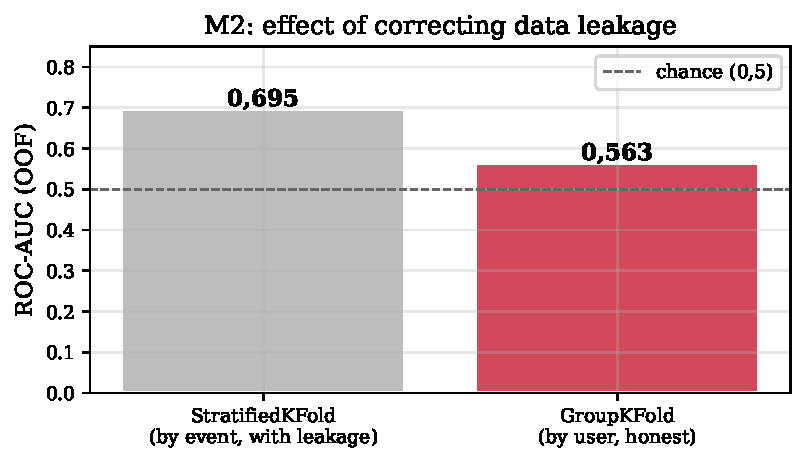
\includegraphics[width=0.6\textwidth]{fig_m2_leakage}
\caption{Efecto de corregir la fuga de datos en M2. La validación por evento (con fuga) inflaba el AUC-ROC; la validación agrupada por usuario da la estimación sin fuga.}
\label{fig:m2_leakage}
\end{figure}

\begin{hallazgo}
El AUC-ROC honesto del modelo demográfico es \textbf{0,56}, no 0,70. El valor inflado era fruto de una
\emph{fuga de datos} (validar por evento en lugar de por usuario). Detectarlo y corregirlo ilustra cómo una
elección de validación inadecuada infla las métricas en problemas con \textit{features} estables por usuario.
\end{hallazgo}

\subsection{Aportación de las variables de producto}
\label{sec:m2-variables}

Se compara primero qué \emph{variables} aportan: la Variante A es un modelo por categoría con solo variables de usuario (el enfoque demográfico tradicional) y la Variante B añade variables de producto (categoría, CPL, atributos de marketing agregados por sector y \textit{embeddings} del texto del asunto del email). La Tabla~\ref{tab:m2_models} y la Figura~\ref{fig:m2_models} resumen los resultados (PR-AUC con intervalo de confianza \textit{bootstrap} al 95\,\%, validación GroupKFold por usuario).

\begin{table}[htbp]
\centering
\caption{M2: aportación de las variables de producto (PR-AUC con IC 95\%, GroupKFold por usuario)}
\label{tab:m2_models}
\begin{tabular}{lccc}
\toprule
\textbf{Estrategia} & \textbf{PR-AUC} & \textbf{IC 95\%} & \textbf{AUC-ROC} \\
\midrule
Baseline popularidad                            & 0,313 & [0,309--0,319] & 0,614 \\
Solo variables de usuario                       & 0,322 & [0,316--0,328] & 0,612 \\
\textbf{Modelo con producto (plano, adoptado)}  & \textbf{0,402} & [0,395--0,410] & \textbf{0,684} \\
\bottomrule
\end{tabular}
\end{table}

\begin{figure}[htbp]
\centering
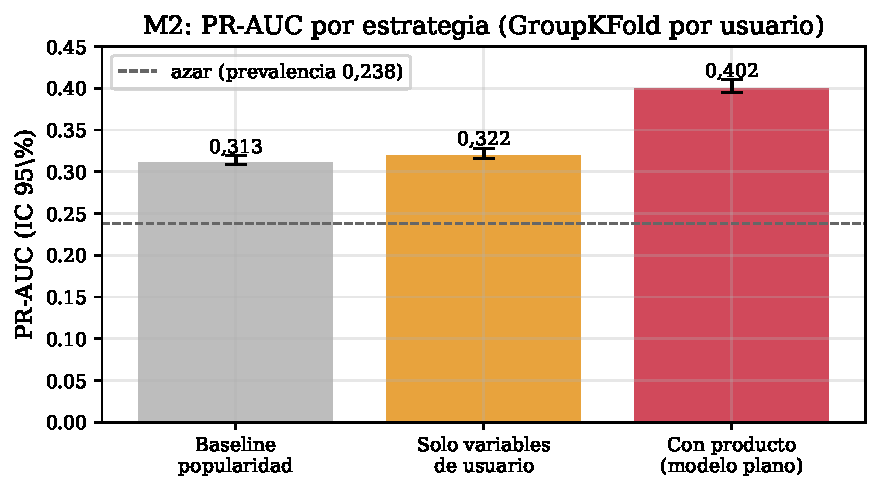
\includegraphics[width=0.8\textwidth]{fig_m2_models}
\caption{PR-AUC de las distintas estrategias de M2 con intervalo de confianza al 95\%. La línea discontinua marca el azar (prevalencia 0,238).}
\label{fig:m2_models}
\end{figure}

El modelo con variables de producto alcanza un PR-AUC de 0,402, muy por encima del modelo de solo-usuario ($\approx+0{,}08$) y del baseline de popularidad ($\approx+0{,}09$), ambas diferencias con $p\approx0$ (test \textit{bootstrap} pareado). El modelo de solo-usuario es estadísticamente indistinguible del baseline de popularidad: el esquema que solo usa variables de usuario apenas personaliza. Los \textit{embeddings} del texto del asunto son una pieza central de esa señal de producto.

\subsection{Comparación de algoritmos y arquitectura}
\label{sec:m2-algos}

Fijadas las variables, se comparan cinco algoritmos (una red neuronal de perceptrón multicapa, LightGBM, HistGradientBoosting, Random Forest y regresión logística) bajo las dos arquitecturas: el modelo \emph{plano} (un único modelo estima $P(\text{click}\mid u,\text{producto})$) y el \emph{jerárquico} ($p_\text{sector}\cdot p_\text{producto}$), todos sobre las mismas particiones GroupKFold por usuario. La Tabla~\ref{tab:m2_algos} recoge el panel de métricas del modelo plano y la Figura~\ref{fig:m2_algos} contrasta ambas arquitecturas.

\begin{table}[htbp]
\centering
\caption{M2: comparación de algoritmos (modelo plano; GroupKFold por usuario; umbral de F1/MCC = prevalencia 0,238). \textit{Brier}: menor es mejor.}
\label{tab:m2_algos}
\begin{tabular}{lccccc}
\toprule
\textbf{Algoritmo} & \textbf{PR-AUC} & \textbf{AUC-ROC} & \textbf{Brier} & \textbf{F1} & \textbf{MCC} \\
\midrule
Random Forest                  & 0,409 & 0,688 & 0,166 & 0,454 & 0,237 \\
\textbf{LightGBM} (adoptado)   & 0,402 & 0,684 & 0,167 & 0,447 & 0,231 \\
HistGradientBoosting           & 0,397 & 0,678 & 0,168 & 0,444 & 0,230 \\
Regresión logística            & 0,391 & 0,673 & 0,169 & 0,441 & 0,216 \\
Red neuronal (MLP)             & 0,378 & 0,661 & 0,174 & 0,432 & 0,207 \\
\bottomrule
\end{tabular}
\end{table}

\begin{figure}[htbp]
\centering
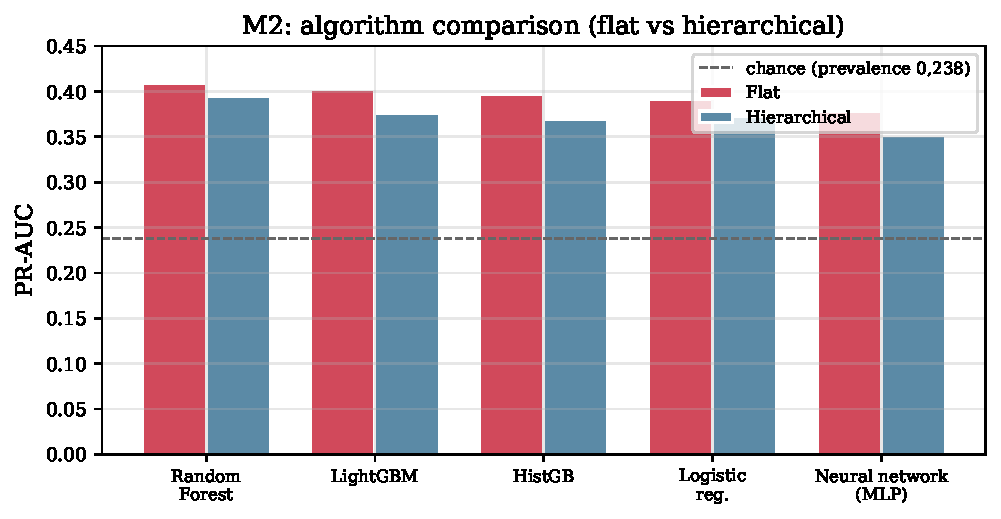
\includegraphics[width=0.78\textwidth]{fig_m2_algos}
\caption{PR-AUC de cada algoritmo en las dos arquitecturas (plano frente a jerárquico). El plano supera al jerárquico en todos los algoritmos; la red neuronal queda última en ambos.}
\label{fig:m2_algos}
\end{figure}

Se extraen tres conclusiones. Primera, la arquitectura plana supera a la jerárquica en los cinco algoritmos ($\Delta$PR-AUC entre $-0{,}014$ y $-0{,}028$): multiplicar por la probabilidad de sector añade error y descalibra las probabilidades (el \textit{Brier} empeora de $\approx0{,}17$ a $\approx0{,}21$); por eso se adopta el modelo plano. Segunda, la red neuronal queda última en ambas arquitecturas, un resultado consistente con la evidencia reciente de que, en datos tabulares, los métodos basados en árboles superan al aprendizaje profundo~\cite{grinsztajn2022}; aquí, con clases desbalanceadas y señal débil, un modelo más complejo no está justificado. Tercera, las diferencias entre los métodos de árboles son pequeñas (Random Forest y LightGBM quedan empatados dentro del intervalo de confianza); se mantiene LightGBM por su manejo nativo de variables categóricas y valores ausentes y por ser el estándar del sector. Ningún algoritmo se despega del entorno de PR-AUC $0{,}40$: el techo lo marcan los datos, no el algoritmo.

Para descartar que la comparación penalizase a algún algoritmo por usar su configuración por defecto (en particular a la red neuronal), se ajustaron los hiperparámetros de cada modelo mediante una búsqueda en rejilla acotada sobre las \emph{mismas} particiones GroupKFold y el modelo plano. Tras el ajuste, el orden se mantiene: Random Forest $0{,}411$ y LightGBM $0{,}409$ siguen empatados a la cabeza, HistGradientBoosting $0{,}406$, y la red neuronal $0{,}395$, pese a mejorar respecto a su configuración por defecto, continúa por debajo de los árboles, seguida de la regresión logística $0{,}392$. El ajuste, por tanto, no altera ninguna de las tres conclusiones ni el modelo adoptado: la ventaja de los árboles sobre la red neuronal es estructural y no un efecto de la parametrización.

\subsection{Interpretabilidad}

La Figura~\ref{fig:m2_importance} muestra la importancia de las variables del modelo adoptado (con variables de producto). Las más relevantes son \texttt{ipa\_class} (poder adquisitivo), \texttt{age\_cat} (edad categorizada) y \texttt{demo\_cluster} (cluster demográfico de M0), que ocupa la tercera posición: el cluster funciona como un resumen compacto del perfil demográfico. Ahora bien, la importancia por número de \textit{splits} refleja cuánto \emph{usa} el modelo una variable, no su valor predictivo real: el estudio de ablación (Tabla~\ref{tab:m2_ablation}) muestra que prescindir del cluster (y del resto de variables de usuario) no reduce el PR-AUC, de modo que su papel es operativo (resolver el arranque en frío) más que predictivo.

\begin{figure}[htbp]
\centering
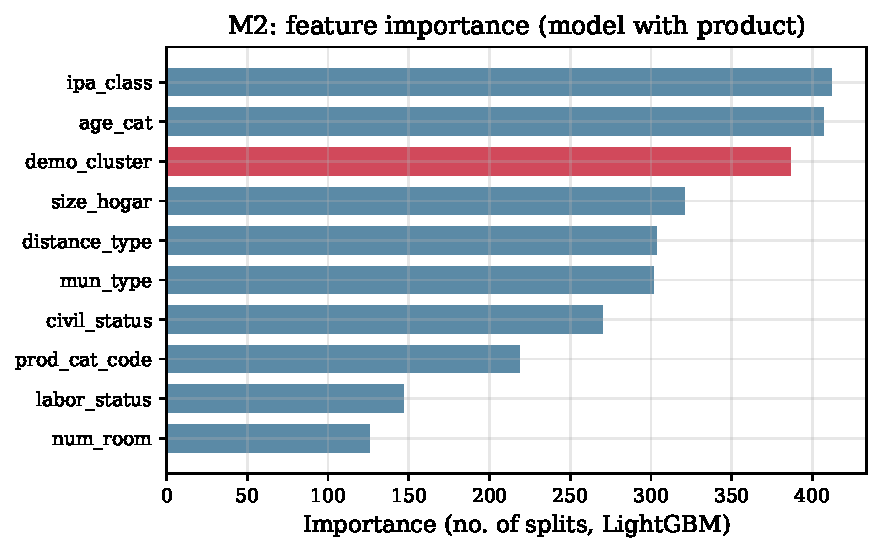
\includegraphics[width=0.72\textwidth]{fig_m2_importance}
\caption{Importancia de variables del modelo de propensión M2 (modelo con variables de producto). El cluster demográfico de M0 (\texttt{demo\_cluster}) es la tercera variable más utilizada.}
\label{fig:m2_importance}
\end{figure}

\subsection{Corrección de prior y sensibilidad}

Las predicciones se calibran al prior real de producción ($\rho_\text{real}=0{,}02$) aplicando la transformación de Dal Pozzolo et al.~\cite{dalpozzolo2015} en escala de \textit{log-odds}, cuyas propiedades (monotonía e invariancia del ranking) se justifican en el Capítulo~\ref{cap:evaluacion}. Tras la corrección, las probabilidades pasan de una media de 0,227 (escala de entrenamiento balanceado) a 0,022, directamente interpretables como estimaciones del comportamiento real (coherentes con el $\approx 2$\,\% de tasa de clic real).

\paragraph{Sensibilidad al prior real.} El valor $\rho_\text{real}=0{,}02$ es una estimación; la tasa de clic real podría situarse en torno al 1\,\% o al 3\,\%. Para comprobar la robustez de las conclusiones se repitió la corrección con esos tres priores (Tabla~\ref{tab:m2_prior}). Por la monotonía de la transformación, el poder de ordenación es invariante: AUC-ROC ($0{,}684$) y PR-AUC ($0{,}402$) no cambian en ninguno de los tres escenarios. Lo único que se desplaza es el nivel absoluto de las probabilidades, cuya media sigue al prior asumido ($1{,}1$\,\% / $2{,}2$\,\% / $3{,}2$\,\%). En otras palabras, la incertidumbre sobre el prior afecta a la \emph{escala} de las probabilidades pero no a la \emph{calidad} del modelo ni al ranking de usuarios, que es lo que se explota en la priorización de envíos. El análisis de ROI a escala de producción (Capítulo~\ref{cap:negocio}) sí emplea estas probabilidades corregidas.

\begin{table}[htbp]
\centering
\caption{M2: sensibilidad de la calibración al prior real de producción ($\rho_\text{real}$). El poder de ordenación (AUC-ROC, PR-AUC) es invariante por ser la corrección monótona; solo cambia el nivel medio de las probabilidades.}
\label{tab:m2_prior}
\begin{tabular}{cccc}
\toprule
\textbf{$\rho_\text{real}$} & \textbf{Media prob. corregida} & \textbf{AUC-ROC} & \textbf{PR-AUC} \\
\midrule
1\,\%          & 0,011 & 0,684 & 0,402 \\
2\,\% (adoptado) & 0,022 & 0,684 & 0,402 \\
3\,\%          & 0,032 & 0,684 & 0,402 \\
\bottomrule
\end{tabular}
\end{table}

\paragraph{Calibración.} Además del orden, interesa que las probabilidades sean realistas. El \textit{Brier score} (menor es mejor) del modelo plano en la escala de entrenamiento es 0,167, y la curva de fiabilidad no presenta desviaciones sistemáticas grandes respecto a la diagonal, lo que indica una calibración razonable. Tras la corrección de \textit{prior}, las probabilidades quedan en la escala de producción ($\approx2\%$), por lo que su \textit{Brier} ya no es comparable con el de la escala balanceada.

\subsection{Modelo \textit{warm} para usuarios con historial}

El M2 descrito es \emph{cold}: usa solo demografía y es válido para cualquier usuario, también nuevos. Para usuarios \emph{con historial} se evaluó un modelo \emph{warm} que añade variables de \textbf{comportamiento} (nº de eventos, clics, \textit{click-rate}, sectores y recencia), calculadas \emph{solo con datos de entrenamiento} para evitar fuga temporal. Para que la comparación no dependa de un único corte temporal arbitrario, se evalúa con validación cruzada temporal (\textit{TimeSeriesSplit} de ventana creciente, 5 cortes sucesivos pasado$\to$futuro), midiendo \emph{cold} y \emph{warm} sobre los eventos de test de usuarios con historial en cada corte. El \emph{warm} mejora sustancialmente al \emph{cold} de forma consistente en los cinco cortes: PR-AUC $0{,}827\pm0{,}031 \to 0{,}943\pm0{,}012$ y AUC-ROC $0{,}810\pm0{,}033 \to 0{,}941\pm0{,}018$ (media\,$\pm$\,desviación típica entre folds), con una mejora media $\Delta$PR-AUC $=+0{,}116\pm0{,}031$ y signo positivo en 5 de 5 cortes. La estabilidad entre folds (desviación pequeña) refuerza que la ganancia es real y no un artefacto de un corte concreto. Esta ganancia aplica solo a la minoría de usuarios con historial; para usuarios nuevos se mantiene el modelo \emph{cold}. Estos valores absolutos no son comparables con el PR-AUC global de M2 (0,402): se miden sobre una subpoblación intrínsecamente más fácil (usuarios recurrentes, con \textit{click-rate} en torno a 0,5 frente a 0,238 global), por lo que lo informativo es la \emph{mejora relativa} del \emph{warm} sobre el \emph{cold} ($\Delta\approx+0{,}12$), no las cifras en sí. En el despliegue, un \textit{endpoint} \texttt{/propensity} selecciona automáticamente \emph{warm} o \emph{cold} según el usuario tenga o no historial.

\subsection{Ablación: ¿qué grupo de variables aporta?}

Para cuantificar el aporte real de cada grupo de variables se realizó un \textbf{estudio de ablación}: se reentrena el modelo (en su forma plana, con predicción \textit{out-of-fold} y validación GroupKFold por usuario) eliminando grupos de variables y midiendo el cambio en PR-AUC con intervalo de confianza \textit{bootstrap}. La Tabla~\ref{tab:m2_ablation} recoge los resultados. Se distinguen las variables \emph{sintéticas muestreadas al azar} (situación laboral, estado civil, vehículo, hogar, habitaciones), la \emph{señal real de usuario} (edad real y variables geográficas derivadas del código postal) y las variables de \emph{producto}.

\begin{table}[htbp]
\centering
\caption{Ablación de M2: PR-AUC por grupo de variables (modelo plano, OOF GroupKFold; azar~=~0,238; n.s.~=~diferencia no significativa)}
\label{tab:m2_ablation}
\begin{tabular}{lrcl}
\toprule
\textbf{Configuración} & \textbf{Nº var.} & \textbf{PR-AUC [IC 95\%]} & \textbf{$\Delta$ vs.\ completo} \\
\midrule
Completo (usuario+producto)      & 39 & 0,402 [0,395--0,410] & --- \\
Sin sintéticas aleatorias        & 34 & 0,402 [0,395--0,410] & $-0{,}001$ (n.s.) \\
\textbf{Solo señal real + producto} & 32 & \textbf{0,407} [0,399--0,415] & $+0{,}004$ (n.s., $p=0{,}06$) \\
Solo producto                    & 28 & 0,398 [0,390--0,406] & $-0{,}005$ (n.s., $p=0{,}07$) \\
Solo usuario (todas)             & 11 & 0,278 [0,273--0,283] & $-0{,}125$ ($p<0{,}001$) \\
\bottomrule
\end{tabular}
\end{table}

Los resultados son claros: (i) eliminar las cinco variables sintéticas muestreadas al azar no cambia la métrica (diferencia no significativa, $p=0{,}68$): no aportan señal; (ii) el mejor modelo numérico conserva \emph{solo} la señal real de usuario (edad y geografía) más el producto, aunque su ventaja sobre el modelo completo tampoco es significativa ($p=0{,}06$); (iii) un modelo con solo variables de producto iguala al modelo completo (diferencia no significativa, $p=0{,}07$), mientras que uno con solo variables de usuario apenas supera el azar (PR-AUC 0,278 vs.\ 0,238; AUC-ROC 0,56). Las variables demográficas sintéticas no aportan poder predictivo: toda la señal reside en el contenido del producto (sector, categoría y texto del asunto). Es la confirmación cuantitativa de la limitación anticipada en el Capítulo~\ref{cap:datos}.

\subsection{¿Bate el modelo a la tasa de clic por categoría?}

Si toda la señal está en el producto, el \textit{baseline} verdaderamente exigente no es la popularidad, sino asignar a cada par la tasa de clic histórica de la categoría del producto (una tabla de frecuencias). Se evalúa \textit{out-of-fold} (la tasa se estima solo con el \textit{train} de cada \textit{fold}, GroupKFold por usuario) y se compara con el modelo plano (Tabla~\ref{tab:m2_ctr}). El modelo supera de forma significativa a esa tabla de frecuencias: PR-AUC 0,402 frente a 0,316 ($\Delta=+0{,}086$, IC 95\% $[+0{,}078,+0{,}094]$, $p\approx0$). La mejora no es residual: confirma que el modelo no se limita a memorizar la propensión media de cada categoría, sino que explota el texto concreto del asunto (vía \textit{embeddings}) para discriminar entre productos de una misma categoría. Es la evidencia que respalda \textbf{H1}. El asunto del email es una variable \emph{legítima} y disponible en el momento de decidir el envío, por lo que usarlo no constituye fuga; y que la ventaja provenga de la semántica del texto o de una codificación más fina de la propia categoría no altera la conclusión operativa: incorporar el asunto mejora el \textit{ranking} de envíos respecto a trabajar solo con la categoría agregada.

\begin{table}[htbp]
\centering
\caption{M2: el modelo plano frente al baseline de tasa de clic por categoría (OOF GroupKFold; azar~=~0,238)}
\label{tab:m2_ctr}
\begin{tabular}{lcc}
\toprule
\textbf{Método} & \textbf{PR-AUC} & \textbf{AUC-ROC} \\
\midrule
Baseline: tasa de clic por sector     & 0,297 & 0,589 \\
Baseline: tasa de clic por categoría  & 0,316 & 0,612 \\
\textbf{Modelo plano (usuario+producto+\textit{embeddings})} & \textbf{0,402} & \textbf{0,684} \\
\bottomrule
\end{tabular}
\end{table}

\section{Modelo inverso: producto \texorpdfstring{$\rightarrow$}{->} perfil}

Se construyó un modelo inverso que, dado un producto, identifica los perfiles de usuario con mayor probabilidad de clic. Metodológicamente se interroga el modelo \emph{forward} de M2 fijando el producto y enumerando todas las combinaciones de un subconjunto de variables (edad, sexo, renta, vehículo, tipo de municipio; 720 combinaciones), de las que se derivan las probabilidades marginales por variable. El efecto del perfil resulta débil: la probabilidad de clic marginal por grupo de edad varía solo entre 0,06 y 0,14 según el producto, lo que indica que es el producto, y no el perfil demográfico, quien determina mayoritariamente la propensión. El método es válido, pero su capacidad informativa está limitada por el carácter sintético de las variables de usuario.

\chapter{Módulo M3 — Recomendador por cluster}
\label{cap:recomendador}

\section{Método}

El recomendador opera a nivel de cluster: el \textit{ranking} de categorías se calcula por segmento comportamental M1 (Capítulo~\ref{cap:segmentacion}) y se sirve a todos sus miembros (un usuario obtiene las recomendaciones de su cluster). Esta decisión nace de la esparsidad del historial. Para justificarla, se parte de un esquema híbrido que combina dos señales de comportamiento para puntuar cada par (usuario, categoría de producto):
\begin{equation}
    s(u, p) = \alpha \cdot \hat{p}_\text{ind}(u, p) + (1-\alpha) \cdot a(s_u, p)
    \label{eq:hybrid}
\end{equation}
donde $a(s_u, p)$ es la afinidad (tasa de clic normalizada) del segmento comportamental $s_u$ del usuario hacia la categoría $p$, y $\hat{p}_\text{ind}(u, p)$ es la tasa de clic histórica del propio usuario en esa categoría. El componente individual se calcula únicamente con los eventos de entrenamiento (no se reutilizan las puntuaciones \textit{out-of-fold} de M2, que mezclaban información de todo el dataset y habrían contaminado la evaluación temporal).

El peso $\alpha$ se ajusta en un conjunto de validación (no en el de test). Con los datos actuales el óptimo es $\alpha=0$: dada la esparsidad (mediana de un evento por usuario), el historial individual no aporta y la señal útil es la afinidad del segmento. Por ello el recomendador prescinde del término individual y sirve directamente el \textit{ranking} del cluster. Para usuarios nuevos sin historial (\textit{cold start}) se emplea la afinidad del cluster demográfico M0.

\subsection*{Evaluación sin fuga}

Como el segmento M1 se construye con todo el historial, evaluarlo sobre un \textit{split} temporal contaminaría la prueba (la pertenencia al cluster ``vería'' el futuro). Por ello, \emph{para evaluar}, el segmento se reconstruye usando solo los eventos de \textit{train} (replicando el pipeline de M1: \texttt{log1p}\,$\rightarrow$\,estandarización\,$\rightarrow$\,PCA\,$\rightarrow$\,KMeans, $k{=}12$), y la afinidad se estima también solo con \textit{train}; en servicio se usa el segmento con todo el historial (uso legítimo, no fuga). La evaluación usa una partición temporal en tres (train / validación / test, 70/10/20 por fecha). Las métricas son Hit Rate@$K$, NDCG@$K$ y MAP@$K$ (Sección~\ref{sec:metricas}), comparadas frente a dos \textit{baselines} (popularidad global y cluster demográfico). El contraste estadístico combina el test de \textbf{Friedman} (diferencia global sobre el NDCG@10 por usuario), \textit{post-hoc} de \textbf{Wilcoxon} pareado y \textbf{McNemar} (sobre los aciertos de HR@5), con corrección de Holm, tamaños de efecto (W de Kendall y rango-biserial) e intervalos de confianza \textit{bootstrap}.

Cada método ordena las categorías por su propio criterio (el recomendador por la \emph{tasa de clic} del segmento y los \textit{baselines} por el \emph{número de clics}). Como las métricas de \textit{ranking} (HR@$K$, NDCG, MAP) dependen únicamente del \emph{orden} de las categorías y no de su escala, la forma de normalizar cada señal no afecta a la comparación.

\section{Resultados}

El recomendador genera el top-5 de categorías a nivel de cluster. La Tabla~\ref{tab:m3_results} y la Figura~\ref{fig:m3_recommender} comparan el recomendador (sin fuga) con los \textit{baselines} sobre 1.573 usuarios con clic en test.

\begin{table}[htbp]
\centering
\caption{M3: recomendador por cluster (segmento M1 sin fuga) frente a baselines (test temporal, $n=1.573$)}
\label{tab:m3_results}
\begin{tabular}{lcccc}
\toprule
\textbf{Método} & \textbf{HR@5} & \textbf{HR@10} & \textbf{NDCG@10} & \textbf{MAP@10} \\
\midrule
\textbf{Baseline popularidad}              & \textbf{0,629} & \textbf{0,806} & \textbf{0,580} & \textbf{0,500} \\
Cluster demográfico                        & 0,629 & 0,789 & 0,572 & 0,496 \\
Recomendador por cluster (M1)              & 0,586 & 0,774 & 0,521 & 0,439 \\
\bottomrule
\end{tabular}
\end{table}

\begin{figure}[htbp]
\centering
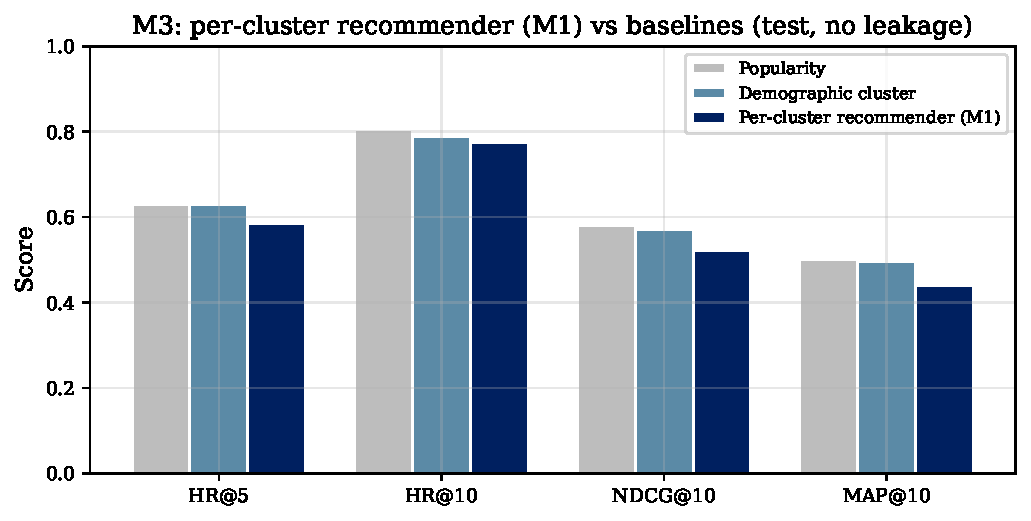
\includegraphics[width=0.85\textwidth]{fig_m3_recommender}
\caption{Comparación del recomendador por cluster (segmento M1, sin fuga temporal) frente a los baselines de popularidad y cluster demográfico (test temporal).}
\label{fig:m3_recommender}
\end{figure}

Una vez eliminada la fuga, el recomendador por cluster no supera a la popularidad en ninguna métrica. La popularidad obtiene mejor HR@5 (0,629 vs.\ 0,586; test de McNemar $p_{\text{Holm}}=3{,}4\times10^{-8}$, el \textit{baseline} gana en 102 usuarios frente a 35), y también mejor HR@10, NDCG@10 y MAP@10. El test de Friedman sobre el NDCG@10 confirma que existen diferencias entre los tres métodos ($\chi^2=142$, $p\approx10^{-31}$), si bien su tamaño de efecto global es pequeño (W de Kendall $=0{,}05$), porque dos de los tres métodos son casi idénticos. El \textit{post-hoc} de Wilcoxon con corrección de Holm lo precisa: popularidad y cluster demográfico son equivalentes entre sí ($p_{\text{Holm}}=0{,}31$; tamaño de efecto rango-biserial $|r|=0{,}06$, despreciable), mientras que ambos superan al recomendador por cluster con un tamaño de efecto grande ($p_{\text{Holm}}<10^{-22}$; $|r|=0{,}65$ y $0{,}54$). La inferioridad del recomendador, por tanto, no es solo estadísticamente significativa: es de magnitud considerable. La ventaja del recomendador comportamental que se observaba con el segmento \emph{contaminado} (HR@5 de 0,687) era un artefacto de fuga (inflación de $\approx0{,}10$ en HR@5).

La lectura es coherente con el resto del trabajo: con un catálogo reducido (25 categorías) y clics muy concentrados, la popularidad es un \textit{baseline} muy difícil de batir, y la señal de segmento no añade poder predictivo sobre ella. El valor del recomendador por cluster es operativo (segmentos interpretables, \textit{ranking} homogéneo y estable por grupo, y una solución natural de arranque en frío), no de mejora de \textit{ranking} frente a popularidad.

\chapter{Módulo M4 — Previsión temporal}
\label{cap:forecast}

\section{Método}

El módulo M4 aplica Prophet \cite{taylor2018forecasting} sobre la serie temporal de clics semanales agregados. El dataset cubre 52 semanas, pero las primeras 30 presentan actividad prácticamente nula (0--50 clics), ya que la campaña no había arrancado. Incluir ese período inactivo en el entrenamiento induce al modelo a aprender una tendencia descendente hacia cero. Para evitarlo, el modelo se entrena exclusivamente sobre el \textbf{período activo}: las 22 semanas a partir de la primera con al menos 50 clics (semana del 28 de julio de 2025), con un rango de 108 a 1.759 clics.

Dado que los datos están agregados por semana (no por día), la estacionalidad semanal de Prophet no aporta señal y se desactiva. La estacionalidad anual tampoco es estimable con menos de seis meses de actividad y se desactiva igualmente. El modelo queda configurado con tendencia lineal, \texttt{changepoint\_prior\_scale}\,=\,0{,}5 para capturar el pico de octubre y la posterior caída, y \texttt{n\_changepoints}\,=\,10. El intervalo de confianza es del 90\,\%. Para la evaluación se emplea primero un hold-out de las últimas 4 semanas y, sobre todo, un \textit{backtest} rolling que se contrasta con baselines ingenuos mediante el test de Diebold-Mariano (Sección~\ref{sec:tests}).

\section{Resultados}

Sobre el hold-out de las últimas 4 semanas, Prophet obtiene MAE\,=\,447 clics/semana, RMSE\,=\,507,7 y MAPE\,=\,73,3\,\%, y predice 259--452 clics/semana para enero--febrero 2026 (Figura~\ref{fig:forecast}). El MAPE está condicionado por un pico atípico en la primera semana del hold-out; las otras tres semanas presentan errores del 2--29\,\%. La amplitud de los intervalos de confianza refleja la incertidumbre de un histórico activo de solo 22 semanas.

\begin{figure}[htbp]
\centering
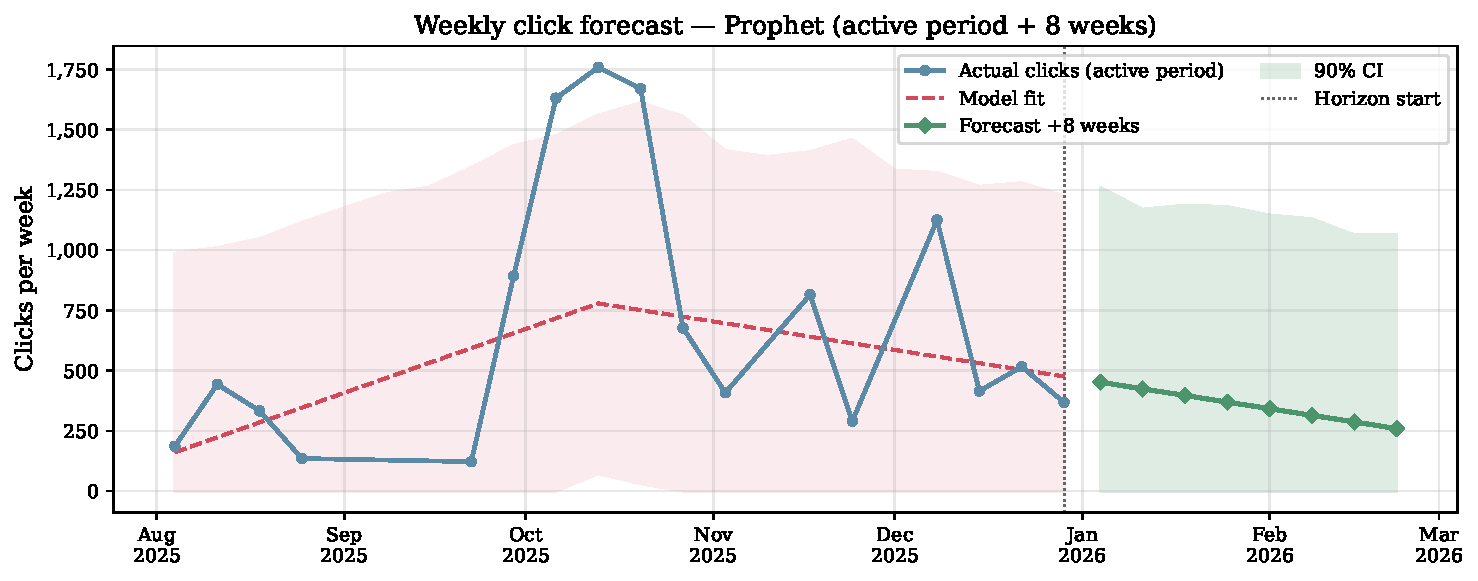
\includegraphics[width=\textwidth]{fig_forecast}
\caption{Forecast de clics semanales con Prophet (M4). Azul: clics reales. Rojo discontinuo: ajuste. Verde: predicción a 8 semanas. La banda sombreada es el intervalo de confianza al 90\%.}
\label{fig:forecast}
\end{figure}

\subsection{Re-auditoría con baselines}

El hold-out de 4 semanas es demasiado corto para una comparación fiable. Se realizó un \textbf{backtest
rolling de 1 paso} (14 orígenes): para cada semana se entrena con todo lo anterior y se predice la
siguiente, comparando Prophet con dos baselines ingenuos (\emph{naïve}: la próxima semana = la última;
y media móvil de 3). La Tabla~\ref{tab:m4_backtest} y la Figura~\ref{fig:m4_backtest} muestran el resultado.

\begin{table}[htbp]
\centering
\caption{M4: error del backtest rolling 1-paso (14 orígenes)}
\label{tab:m4_backtest}
\begin{tabular}{lcc}
\toprule
\textbf{Modelo} & \textbf{MAE} & \textbf{RMSE} \\
\midrule
Prophet        & 749,7 & 874,7 \\
\textbf{Naïve} & \textbf{502,3} & \textbf{604,6} \\
Media móvil 3  & 583,7 & 703,7 \\
\bottomrule
\end{tabular}
\end{table}

\begin{figure}[htbp]
\centering
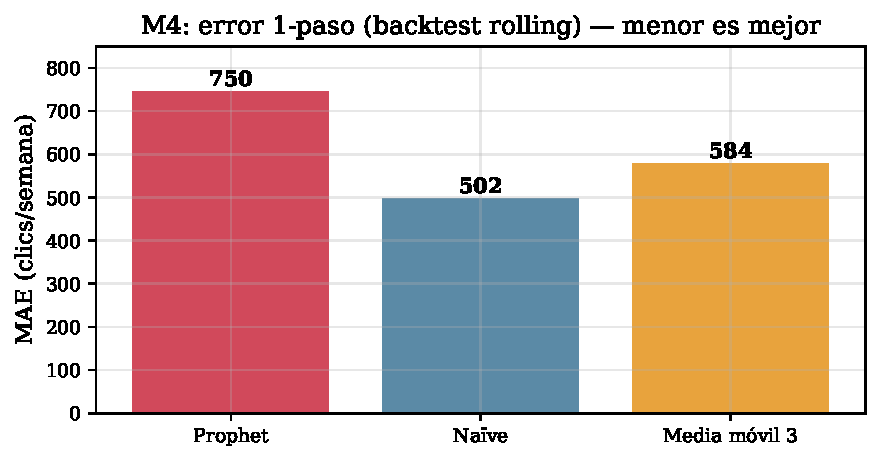
\includegraphics[width=0.62\textwidth]{fig_m4_backtest}
\caption{Error medio absoluto (MAE) del backtest rolling 1-paso de M4. Los baselines ingenuos baten a Prophet.}
\label{fig:m4_backtest}
\end{figure}

El resultado es claro en el error puntual: en esta serie corta y volátil, \textbf{los baselines ingenuos baten
a Prophet} (MAE 750 frente a 502 del \emph{naïve}). Ahora bien, con solo 14 orígenes el test de
Diebold-Mariano requiere la \textbf{corrección de Harvey-Leybourne-Newbold} (factor de muestra pequeña y $t$ de
Student con $n-1$ grados de libertad); aplicada, la diferencia resulta \textbf{marginal} (vs.\ \emph{naïve}
$p=0{,}059$; vs.\ media móvil $p=0{,}073$): no alcanza la significación al 5\,\%, lo cual es coherente con un
histórico tan corto. La lectura honesta es que el simple ``la próxima semana será como la última'' iguala o
supera a Prophet ---cuya flexibilidad de tendencia sobreajusta con tan pocos datos---, aunque la evidencia es
\emph{sugestiva} más que concluyente por la escasez de puntos.


\part{Application and closing}
\chapter{Despliegue y análisis de negocio}
\label{cap:negocio}

Este capítulo cierra el pipeline con su vertiente aplicada: un ejemplo de despliegue del sistema como servicio y un análisis del retorno de la inversión (ROI) que traduce las predicciones de propensión a una decisión de negocio.

\section{Despliegue}

Como demostración de productización se implementó una API REST de ejemplo (FastAPI) que sirve las recomendaciones: para un usuario conocido devuelve su top-5 precalculado en \textit{batch}; para un usuario nuevo aplica el pipeline de arranque en frío (\textit{features} $\rightarrow$ cluster demográfico $\rightarrow$ afinidades del cluster); y recurre a la popularidad como último recurso. La API expone además un \textit{endpoint} \texttt{/propensity} que, a partir del modelo plano de M2, devuelve para un usuario o un perfil la probabilidad de clic desglosada por sector y por producto (probabilidades independientes \textit{one-vs-rest}, corregidas al prior real), que es la forma operativa de decidir qué enviar a quién. No constituye un servicio de producción, sino una ilustración del flujo de inferencia.

\subsection{Especificación de la API}

La API expone cinco \textit{endpoints} (Tabla~\ref{tab:api}). Las entradas de los métodos \texttt{POST} son un objeto JSON con el perfil del usuario, cuyos campos categóricos se introducen como texto legible (p.\,ej.\ \texttt{mun\_type="Ciudad"}); la API realiza internamente la codificación numérica que espera el modelo, garantizando el mismo orden de variables que en el entrenamiento. Todos los campos son opcionales y tienen un valor por defecto, y las entradas fuera de dominio se rechazan automáticamente con un error 422.

\begin{table}[htbp]
\centering
\caption{Endpoints de la API de ejemplo}
\label{tab:api}
\small
\begin{tabular}{lll}
\toprule
\textbf{Método y ruta} & \textbf{Entrada} & \textbf{Salida} \\
\midrule
\texttt{GET /health}                 & ---            & estado y nº de artefactos \\
\texttt{GET /recommend/\{user\_id\}}  & id de usuario  & top-5 de categorías del cluster \\
\texttt{POST /recommend/coldstart}    & perfil (JSON)  & top-5 vía cluster demográfico \\
\texttt{GET /propensity/\{user\_id\}} & id de usuario  & prob.\ de clic por sector y producto \\
\texttt{POST /propensity}             & perfil (JSON)  & prob.\ de clic por sector y producto \\
\bottomrule
\end{tabular}
\end{table}

El \textit{endpoint} \texttt{/propensity} devuelve, para un usuario o perfil, la probabilidad de clic de cada uno de los 13 sectores y las 25 categorías de producto (cada producto acompañado de su sector), ya corregida al \textit{prior} real ($\approx 2$\,\%). Son probabilidades independientes (\textit{one-vs-rest}): cada una responde ``¿cuál es la probabilidad de clic si le envío esto?'' y no suman uno. Un ejemplo de respuesta para el producto más propenso de un perfil dado sería \texttt{\{"producto":"car\_leasing","sector":"motor","p\_click":0.046\}}.

\section{Análisis de retorno de la inversión (ROI)}
\label{sec:roi}

Para evaluar el valor de negocio, se compara el ROI de la campaña registrada en la base de datos
(``enviar a todos'') frente a nuestro modelo (``priorizar''). Se interpreta el CPL como el beneficio
que deja cada clic; el beneficio de un producto es (clics $\times$ CPL). El coste de enviar un email se
analiza bajo tres estructuras, todas por email enviado: \emph{fijo} (un valor igual para todos los
productos, 1\,\euro), \emph{variable} (un porcentaje del CPL del producto; se comparan 20\,\%, 30\,\% y
40\,\%) y \emph{mixto} (una base fija de 0,50\,\euro\ más el 15\,\% del CPL). El modelo envía un email solo
si su beneficio esperado ($p_\text{model}\times\text{CPL}$) supera su coste marginal; en el caso variable
esta regla equivale exactamente a $p_\text{model}\ge\text{porcentaje}$. La Tabla~\ref{tab:roi_producto} recoge el ROI agregado por estructura de coste.

\begin{table}[htbp]
\centering
\caption{ROI agregado: campaña de la BD vs.\ modelo de priorización, por estructura de coste por email}
\label{tab:roi_producto}
\small
\begin{tabular}{lrrrrr}
\toprule
\textbf{Estructura de coste} & \textbf{ROI BD} & \textbf{ROI modelo} & \textbf{Mejora} & \textbf{Emails} & \textbf{Prod.\ mejoran} \\
\midrule
Fijo (1\,\euro/email)         &    101\% & \textbf{148\%} & \textbf{+47\,pts} & 72,0\% & 21/25 \\
Variable 20\,\% CPL           &     18\% & \textbf{67\%}  & \textbf{+49\,pts} & 48,2\% & 22/25 \\
Variable 30\,\% CPL           & $-$21\%  & \textbf{37\%}  & \textbf{+58\,pts} & 24,3\% & 21/25 \\
Variable 40\,\% CPL           & $-$41\%  & \textbf{21\%}  & \textbf{+62\,pts} & 12,2\% & 19/25 \\
Mixto (0,50\,\euro\ + 15\,\% CPL) & 13\% & \textbf{65\%}  & \textbf{+52\,pts} & 41,7\% & 21/25 \\
\bottomrule
\end{tabular}
\end{table}

A diferencia de la estructura puramente fija \emph{por producto} (donde enviar a todos sería óptimo porque
el coste no depende del volumen), al ser el coste marginal por email la priorización aporta valor en
las tres estructuras: el modelo deja de enviar los emails cuyo beneficio esperado no cubre su coste y descarta
productos deficitarios (CPL bajo y poca propensión, p.\,ej.\ \texttt{life\_insurance}, \texttt{sweepstakes},
\texttt{loan}). Cuanto más caro es el email (porcentajes altos del CPL), más selectivo se vuelve el modelo
(del 72\,\% de envíos con coste fijo al 12\,\% con el 40\,\% del CPL). La Figura~\ref{fig:roi} resume el ROI
agregado en todos los escenarios.

\begin{figure}[htbp]
\centering
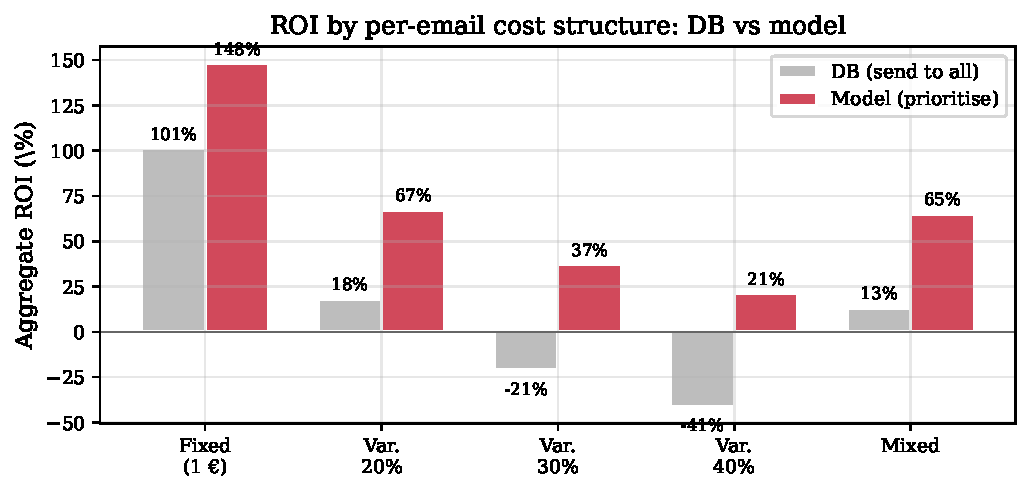
\includegraphics[width=0.75\textwidth]{fig_roi}
\caption{ROI agregado según la estructura de coste por email: campaña de la BD frente al modelo de priorización.}
\label{fig:roi}
\end{figure}

El caso \emph{fijo} (1\,\euro/email) mejora el ROI de 101\,\% a 148\,\% enviando al 72\,\% de mayor
propensión: filtra el $\approx$28\,\% de envíos cuyo beneficio esperado no cubre el coste. En el caso
\emph{variable}, la regla $p_\text{model}\ge\text{porcentaje}$ es más exigente cuanto mayor es el
porcentaje: enviar a todos resulta \emph{deficitario} a partir del 30\,\% (ROI negativo), porque el coste por
email es alto frente a la tasa de clic del \emph{sample} ($\approx$24\,\%); el modelo lo rescata a
positivo en todos los casos (del $-$21\,\% al $+$37\,\% con el 30\,\%; del $-$41\,\% al $+$21\,\% con el
40\,\%), a costa de enviar cada vez menos. El caso \emph{mixto} mejora de 13\,\% a 65\,\%.

\begin{hallazgo}
Bajo coste marginal por email, el modelo de priorización mejora el ROI en las tres
estructuras de coste (p.\,ej.\ 101\,\%\,$\to$\,148\,\% en el caso fijo): filtra los envíos cuyo beneficio
esperado no cubre su coste y rescata a positivo incluso los escenarios donde enviar a todos es
deficitario (variable $\geq$30\,\%). El grado de filtrado depende del coste por email: del $\approx$28\,\% de
envíos descartados con coste fijo al $\approx$88\,\% con el 40\,\% del CPL. La elección del punto de operación
depende del objetivo de negocio: maximizar la \emph{eficiencia} (\euro\ por clic) o el \emph{alcance} (clics
totales).
\end{hallazgo}

\paragraph{Apunte: propensión, no incrementalidad.} El modelo estima la \emph{propensión} (probabilidad de clic), no la \emph{incrementalidad} o \textit{uplift} (el efecto \emph{causal} del envío): el ROI atribuye al email todos los clics de los usuarios priorizados, aunque algunos habrían ocurrido igualmente sin recibirlo. Cuantificar ese efecto causal exigiría un grupo de control (usuarios comparables no impactados), que estos datos (solo envíos registrados) no permiten construir. El matiz afecta a la lectura \emph{absoluta} de las cifras, no a la conclusión relativa: como ``enviar a todos'' y ``priorizar'' se evalúan bajo el mismo supuesto, la comparación entre ambas es justa y el modelo mejora el ROI en todos los escenarios. La estimación de la incrementalidad se deja como línea de trabajo futuro.

\subsection{ROI a escala de producción}

Las cifras anteriores se calculan sobre la muestra balanceada de evaluación (tasa de clic $\approx$24\,\%); comparan, por tanto, \emph{en términos relativos} ``enviar a todos'' frente a ``priorizar''. Para estimar el ROI \emph{absoluto} de producción se repondera cada envío al prior real ($\approx$2\,\%) y se decide con la probabilidad \emph{corregida} (enviar si $p_\text{real}\cdot\text{CPL}\ge$ coste marginal). El resultado (Tabla~\ref{tab:roi_prod}) es ilustrativo.

\begin{table}[htbp]
\centering
\caption{ROI a escala de producción (prior real $\approx$2\,\%): campaña de la BD vs.\ modelo}
\label{tab:roi_prod}
\begin{tabular}{lrrr}
\toprule
\textbf{Estructura de coste} & \textbf{ROI ``enviar a todos''} & \textbf{ROI modelo} & \textbf{Emails enviados} \\
\midrule
Fijo (1\,\euro/email)         & $-$83\% & \textbf{$-$1\%} & 0,2\% \\
Variable 20\,\% CPL           & $-$90\% & $-$51\%        & $\approx$0\% \\
Variable 30\,\% CPL           & $-$93\% & $-$100\%       & $\approx$0\% \\
Variable 40\,\% CPL           & $-$95\% & ---            & 0\% \\
Mixto (0,50\,\euro\ + 15\,\% CPL) & $-$91\% & $-$37\%   & $\approx$0\% \\
\bottomrule
\end{tabular}
\end{table}

A una tasa de clic real del 2\,\%, enviar a todos pierde dinero en todas las estructuras ($-$83\,\% a $-$95\,\%): con un beneficio esperado por email de $0{,}02\times8{,}5\approx0{,}17$\,\euro\ frente a costes de 1\,\euro\ o más, el canal es estructuralmente deficitario. Ni siquiera el caso más favorable (coste fijo bajo) llega a ser rentable: el modelo lo lleva de $-$83\,\% a apenas el punto de equilibrio ($\approx-1$\,\%), enviando solo al 0,2\,\% más propenso. Bajo coste variable (un porcentaje del CPL) la regla exige $p_\text{real}\ge$ porcentaje (20--40\,\%), inalcanzable cuando el percentil 90 de $p_\text{real}$ es 4,7\,\%; apenas se envía y el canal sigue siendo deficitario. La lectura de negocio es clara: a escala real, el targeting es imprescindible pero no suficiente, y lo que domina la rentabilidad es la economía unitaria (coste por email frente a CPL). Para el objetivo de este trabajo, demostrar la \emph{metodología} de un proyecto orientado al ROI, este resultado es tan valioso como uno positivo: el proceso cuantifica la restricción económica vinculante y evita recomendar una campaña deficitaria, lo que es en sí una decisión de negocio fundamentada. Que el pipeline exponga este hecho en lugar de ocultarlo es, precisamente, parte de su valor.

\chapter{Conclusiones}
\label{cap:conclusiones}

\section{Discusión}

Los módulos anteriores comparten una lección de método. El diseño inicial trataba la \emph{estimación de propensión} y la \emph{recomendación} como un mismo problema y asumía, sin contrastarlo, que el perfil demográfico del usuario sería la variable determinante. Separar ambos problemas y exigir que fuese la evidencia, y no la intuición de partida, quien decidiese qué señal importa en cada uno cambió el diagnóstico. Qué señal resulta finalmente útil para cada tarea se detalla en la sección siguiente; lo relevante aquí es que esa pregunta se respondió midiendo, no suponiendo.

La segunda lección es que la forma de validar puede pesar más que la elección del modelo. La fuga de datos en el módulo de propensión no nacía de un fallo del algoritmo, sino de un esquema de validación que dejaba al mismo usuario en entrenamiento y prueba; corregirla rebajó el rendimiento aparente del modelo demográfico a su valor realista. En el recomendador ocurrió algo parecido: reconstruir el segmento usando solo datos de entrenamiento eliminó una ventaja que era un artefacto. Comparar cada modelo contra \textit{baselines} triviales y respaldar cada afirmación con tests pareados (bootstrap, McNemar, Wilcoxon) y corrección por comparaciones múltiples evitó dar por buenas mejoras inexistentes.

La tercera lección es que, en este problema, lo que más limita el rendimiento no es el modelado sino los datos. Las variables demográficas del usuario son sintéticas, muestreadas de distribuciones agregadas, y aportan poca señal individual; ese techo acota lo que cualquier algoritmo puede lograr y condiciona la lectura de todos los módulos.

\begin{hallazgo}
\textbf{Conclusión central.} La señal útil para la \emph{propensión} reside en el contenido del producto
(sector, categoría y texto del asunto); la útil para \emph{recomendar} reside en el \emph{comportamiento}
del usuario, no en su perfil demográfico. Las variables demográficas sintéticas marcan el techo del
rendimiento, por lo que el valor del trabajo está en la metodología.
\end{hallazgo}

\section{Conclusiones principales}

Este trabajo ha desarrollado un \textit{framework} integral de aprendizaje automático para la optimización de campañas de email marketing en el mercado español, cubriendo el ciclo completo desde la ingesta de datos brutos hasta la recomendación personalizada, la previsión de demanda y un ejemplo de despliegue. Más allá de los módulos, la principal aportación es metodológica: un pipeline reproducible que toma cada decisión de forma justificada (validación sin fuga, comparación frente a \textit{baselines} triviales antes de adoptar un modelo, corrección del sesgo de muestreo y contraste estadístico) y que distingue con evidencia qué señal es útil para cada problema, qué modelo merece desplegarse y a qué coste. Su valor no reside en una métrica de exactitud máxima, sino en un proceso disciplinado que reporta también lo que \emph{no} funciona. Leído así, el trabajo funciona como una guía para desarrollar un proyecto de datos orientado a maximizar el ROI: cada etapa muestra qué construir, cómo validarlo y cómo fundamentar la decisión de desplegar o no, incluida la de \emph{no} lanzar una campaña cuando la economía del canal no lo justifica.

De las cuatro hipótesis falsables planteadas en la introducción, se \emph{confirma} \textbf{H1} (las variables de producto mejoran significativamente la propensión, $p\approx0$) y se \emph{rechazan} las otras tres: H2 (el estudio de ablación muestra que las demográficas sintéticas no aportan poder predictivo), H3 (el recomendador por cluster no supera a la popularidad) y H4 (Prophet no mejora a los baselines ingenuos). Tres hipótesis rechazadas no son un fracaso: delimitan con evidencia dónde reside, y dónde no, la señal útil del problema.

Propensión y recomendación son problemas distintos, y la señal útil difiere según el objetivo. Para estimar la \emph{propensión} al clic, las variables de \emph{producto} (el sector, la categoría y, sobre todo, el texto del asunto del email codificado mediante \textit{embeddings}) aportan de forma estadísticamente significativa: el modelo con variables de producto (PR-AUC 0,402) supera tanto al modelo basado solo en variables de usuario como a los baselines de popularidad y de tasa de clic por categoría (véase el Capítulo~\ref{cap:propension}), lo que confirma que no se limita a memorizar la propensión media de cada categoría, sino que explota el texto del asunto. Una comparación de cinco algoritmos y dos arquitecturas (plano frente a jerárquico) confirma que el modelo plano supera al jerárquico en todos los algoritmos y que la red neuronal no aporta en datos tabulares con señal débil; el techo de rendimiento ($\approx0{,}40$ de PR-AUC) lo marcan los datos, no el algoritmo. Para \emph{recomendar}, en cambio, lo que discrimina es el \emph{comportamiento} del usuario (su segmento), no su perfil demográfico.

La validación cambia las conclusiones. La detección y corrección de una fuga de datos en M2 (el uso de validación cruzada por evento en lugar de agrupada por usuario) reveló que el rendimiento real del modelo demográfico (AUC-ROC 0,563) era muy inferior al inicialmente estimado (0,695). Este hallazgo constituye una contribución metodológica: ilustra cómo una elección de validación inadecuada puede inflar de forma engañosa las métricas en problemas donde las features son atributos estables del usuario.

El recomendador por cluster aporta valor operativo, no predictivo. Sirve sus recomendaciones \emph{a nivel de cluster} (segmento comportamental M1). Al evaluarlo sin fuga, reconstruyendo el segmento solo con datos de entrenamiento, \emph{no supera} a la popularidad en ninguna métrica (HR@5 0,586 frente a 0,629 a favor de la popularidad), un resultado confirmado por un test de Friedman seguido de Wilcoxon con corrección de Holm; la ventaja aparente del segmento contaminado era un artefacto de fuga temporal. Algo análogo ocurre con el cluster demográfico de M0: es la variable más \emph{usada} por M2 (3.ª por número de \textit{splits}), pero el estudio de ablación demuestra que su aporte predictivo es nulo, ya que prescindir de él y del resto de variables de usuario no reduce el PR-AUC. El valor de ambos es, por tanto, \emph{operativo}: segmentos interpretables, \textit{ranking} homogéneo por grupo y solución natural de arranque en frío, asignando a cada usuario nuevo las afinidades de su grupo. No mejoran el \textit{ranking} sobre una popularidad que, con un catálogo de 25 categorías y clics concentrados, resulta un \textit{baseline} muy fuerte.

El módulo M4 produce predicciones en el rango 259--452 clics/semana para enero--febrero 2026, con intervalos de confianza amplios coherentes con un histórico activo de solo 22 semanas. Una re-auditoría mediante \textit{backtest} rolling de 1 paso revela, además, que Prophet no supera a baselines ingenuos (naïve y media móvil): su error es mayor (MAE 750 frente a 502) aunque, con solo 14 orígenes y la corrección de muestra pequeña de Harvey-Leybourne-Newbold, la diferencia no alcanza significación al 5\% (Diebold-Mariano $p\approx0{,}06$), por lo que la evidencia es sugestiva, no concluyente. En una serie corta y volátil, ``la próxima semana será como la última'' iguala o supera a Prophet, un resultado negativo que cuestiona su valor añadido en este contexto.

Para usuarios con historial, un modelo \emph{warm} que añade su comportamiento pasado mejora la propensión de forma notable y consistente (PR-AUC $0{,}83\,\to\,0{,}94$, con mejora en los cinco cortes de una validación cruzada temporal), frente al modelo demográfico \emph{cold} válido para usuarios nuevos. Las probabilidades del modelo plano están razonablemente calibradas (\textit{Brier} 0,167 en la escala de entrenamiento). El modelo plano de propensión se expone en la API de ejemplo mediante un \textit{endpoint} \texttt{/propensity} que, dado un usuario conocido o un perfil nuevo, devuelve la probabilidad de clic desglosada por sector y por producto (corregida al prior real).

El análisis económico, interpretando el CPL como beneficio por clic, muestra que, bajo coste marginal por email, priorizar los envíos con el modelo mejora el ROI en las tres estructuras de coste analizadas (fijo, variable y mixto; por ejemplo, de 101\,\% a 148\,\% en el caso fijo), descartando los envíos cuyo beneficio esperado no cubre su coste y rescatando a positivo incluso los escenarios donde enviar a todos es deficitario. El punto de operación óptimo depende del objetivo de negocio (eficiencia frente a alcance). Ahora bien, esa comparación se hace sobre la muestra balanceada; al recalcular el ROI a escala de producción (reponderando al prior real del 2\,\% y decidiendo con la probabilidad corregida), el panorama es más crudo: enviar a todos pierde dinero en todas las estructuras y ni siquiera el mejor caso (coste fijo bajo) llega a ser rentable, pues el modelo lo lleva al punto de equilibrio ($\approx-1$\,\%, frente al $-$83\,\% de enviar a todos) con una fracción mínima de envíos. La lectura de negocio es que, a tasas de clic realistas, el targeting es imprescindible pero la rentabilidad la dicta la economía unitaria (coste por email frente a CPL).

\section{Limitaciones}

\begin{enumerate}
    \item \textbf{Variables sintéticas.} Las variables demográficas enriquecidas (situación laboral, estado civil, tamaño del hogar, habitaciones y tenencia de vehículo) son imputaciones estocásticas a partir de distribuciones agregadas del INE; no se observan a nivel individual. Un estudio de ablación lo confirma cuantitativamente: un modelo de propensión con \emph{solo} variables de producto iguala al modelo completo, mientras que uno con \emph{solo} variables de usuario apenas supera el azar (PR-AUC 0,278 vs.\ 0,238). Esto fija un techo bajo a la señal demográfica y explica por qué tanto el modelo inverso como el recomendador demográfico tienen poca capacidad discriminativa. Es la limitación dominante del trabajo.

    \item \textbf{Esparsidad extrema.} El 83,8\% de los usuarios tiene un único evento, lo que impide construir perfiles comportamentales fiables para la mayoría de la base y explica que el componente de historial individual del recomendador no aporte (peso $\alpha=0$).

    \item \textbf{Catálogo reducido.} Con solo 25 categorías de producto y clics concentrados en unas pocas, el baseline de popularidad es muy fuerte, lo que limita el margen de mejora medible de cualquier recomendador.

    \item \textbf{Tamaño de la subpoblación \textit{warm}.} El modelo \emph{warm} solo aporta a los usuarios con historial, que son minoría; para la mayoría (un evento) sigue rigiendo el límite de la señal demográfica sintética.

    \item \textbf{Previsión con histórico corto.} Prophet dispone de solo 22 semanas de actividad, lo que limita la fiabilidad del forecast más allá de pocas semanas y produce intervalos de confianza amplios. M4 se re-auditó con un \textit{backtest} rolling y el test de Diebold-Mariano (con corrección de muestra pequeña de Harvey-Leybourne-Newbold), pero la escasez de orígenes (14) limita la potencia estadística, por lo que la evidencia es sugestiva.

    \item \textbf{El modelo capta solo una etapa del embudo (clic dado apertura).} Un correo atraviesa dos filtros sucesivos: envío\,$\rightarrow$\,apertura\,$\rightarrow$\,clic. Como los datos solo contienen correos \emph{abiertos}, la variable objetivo es ``clic \emph{dado que} se abrió'': el modelo estima $P(\text{clic}\mid\text{apertura})$ y no modela la primera etapa (la probabilidad de que el correo llegue a abrirse). En consecuencia, la corrección de \textit{prior} al 2\,\% y el ROI ``por email enviado'' son exactos solo si la tasa de apertura es parecida entre productos; si un producto se abre mucho más que otro, su propensión real por envío diferiría aunque su clic-dado-apertura fuese idéntico. La extensión natural es un modelo en dos fases (uno para la apertura y otro para el clic) cuyo producto, $P(\text{abre})\cdot P(\text{clic}\mid\text{abre})$, recupera la propensión real por email enviado.
\end{enumerate}

\section{Trabajo futuro}

\begin{enumerate}
    \item \textbf{Datos reales en lugar de imputados.} La mejora con mayor impacto potencial es sustituir las variables demográficas sintéticas por observaciones reales (CRM, comportamiento en la web del anunciante). Todo el pipeline rendiría más sin cambios en el modelado.

    \item \textbf{Profundizar el modelo \textit{warm}.} El modelo \emph{warm} básico ya se implementó y evaluó (mejora demostrada para usuarios con historial). Como extensión, incorporar más señales de comportamiento (secuencia temporal de interacciones, recencia por sector) y un esquema de actualización incremental.

    \item \textbf{Mejorar la previsión temporal.} La re-auditoría mostró que Prophet no bate a baselines ingenuos en esta serie. Como alternativa, explorar modelos específicos para series cortas (suavizado exponencial, ARIMA con diagnóstico) o incorporar covariables de campaña (nº de envíos, presupuesto) como regresores externos.

    \item \textbf{Evaluación en producción e incrementalidad.} La validación \textit{offline} tiene límites conocidos en recomendación; un test A/B controlado (con grupo de envío y grupo de control) mediría el impacto real sobre la tasa de clic y el retorno de inversión, y permitiría estimar la \emph{incrementalidad} (\textit{uplift}) de cada envío, es decir, su efecto causal, que el análisis de ROI no captura al medir propensión y no efecto causal.
\end{enumerate}


\appendix
\chapter{Reproducibilidad}
\label{ap:reproducibilidad}

Este apéndice reúne la información necesaria para reproducir los resultados del trabajo: entorno de ejecución, versiones de las librerías, semillas aleatorias, orden de ejecución de los \textit{notebooks}, organización de los datos y esquema de validación. El objetivo es que un tercero pueda regenerar el \textit{pipeline} completo y obtener las mismas cifras. El código fuente completo (sin los datos de campaña, que son privados) está disponible en el repositorio \url{https://github.com/germangg26/TFM}.

\section{Entorno y gestión de dependencias}

El proyecto se desarrolla en \textbf{Python 3.12} (fijado en el fichero \texttt{.python-version}). La gestión de dependencias se realiza con \textbf{uv}, que registra las versiones exactas en \texttt{uv.lock}; la instalación completa del entorno se obtiene con \texttt{uv sync}. La Tabla~\ref{tab:versiones} recoge las versiones de las librerías principales empleadas.

\begin{table}[htbp]
\centering
\caption{Versiones de las librerías principales.}
\label{tab:versiones}
\begin{tabular}{ll}
\toprule
\textbf{Librería} & \textbf{Versión} \\
\midrule
numpy                 & 2.4.4 \\
pandas                & 3.0.3 \\
scikit-learn          & 1.8.0 \\
lightgbm              & 4.6.0 \\
tensorflow            & 2.21.0 \\
sentence-transformers & 5.5.1 \\
prophet               & 1.3.0 \\
scipy                 & 1.17.1 \\
matplotlib            & 3.10.9 \\
seaborn               & 0.13.2 \\
\bottomrule
\end{tabular}
\end{table}

\section{Semillas aleatorias}

Todos los procesos con componente aleatoria fijan la semilla \textbf{42} para garantizar la reproducibilidad: el muestreo de datos (\texttt{random\_state=42}), la inicialización de \textit{numpy} (\texttt{np.random.seed(42)}), las particiones de validación cruzada, el \textit{bootstrap} (\texttt{RandomState(42)}, 1000 repeticiones) y los modelos (\texttt{random\_state=42} en LightGBM, \textit{scikit-learn} y el autoencoder). En el autoencoder (M0) se activa además el determinismo de operaciones de TensorFlow (\texttt{TF\_ENABLE\_ONEDNN\_OPTS=0} y \textit{enable\_op\_determinism}) para que la incrustación sea idéntica entre ejecuciones.

\section{Orden de ejecución de los \textit{notebooks}}

El \textit{pipeline} se ejecuta en el orden indicado (Tabla~\ref{tab:pipeline}); cada \textit{notebook} consume los ficheros que generaron los anteriores (todos en \texttt{data/processed/}).

\begin{table}[htbp]
\centering
\caption{Orden de ejecución y artefactos principales.}
\label{tab:pipeline}
\begin{tabular}{lll}
\toprule
\textbf{Notebook} & \textbf{Función} & \textbf{Salida principal} \\
\midrule
\texttt{01\_clean}             & Limpieza y muestreo 1:1     & \texttt{users/events/products.csv} \\
\texttt{02\_geo}               & Enriquecimiento geográfico  & actualiza \texttt{users.csv} \\
\texttt{03\_users}             & Enriquecimiento demográfico & \texttt{users.csv} final \\
\texttt{04\_eda}               & Análisis exploratorio       & (figuras) \\
\texttt{05\_demo\_segmentation} & M0: segmentación demográfica & \texttt{users\_demo\_segments.csv} \\
\texttt{05b\_k\_stability}      & Diagnóstico de estabilidad de $k$ & (diagnóstico) \\
\texttt{06\_segmentation}      & M1: segmentación conductual & \texttt{users\_segmented.csv} \\
\texttt{07\_propensity}        & M2: modelo de propensión    & \texttt{propensity\_scores.csv} \\
\texttt{08\_recommender}       & M3: recomendador por cluster & \texttt{recommendations.csv} \\
\texttt{09\_forecast}          & M4: \textit{forecast} semanal & \texttt{forecast\_clicks.csv} \\
\texttt{10\_inverse\_profile}  & Modelo inverso producto$\to$perfil & (perfiles) \\
\texttt{11\_roi}               & Análisis de ROI             & (tablas de ROI) \\
\bottomrule
\end{tabular}
\end{table}

Dependencias relevantes: \texttt{07\_propensity} usa el \textit{cluster} demográfico de \texttt{05}; \texttt{08\_recommender} usa el segmento conductual de \texttt{06}; \texttt{11\_roi} usa las probabilidades de \texttt{07}. El \textit{forecast} (\texttt{09}) es independiente de la tabla de usuarios.

\section{Datos}

Los datos brutos de campaña (\texttt{data/raw/}) no se versionan por su tamaño y carácter privado. De los $\approx 2$ millones de eventos originales (2.026.166) se toma una \textbf{muestra balanceada 1:1} (todos los clics más un número igual de no-clics), lo que da una prevalencia de entrenamiento de $\approx 0{,}238$; el prior real de producción ($\approx 2$\,\%) se restaura mediante la corrección de \textit{prior} (véase el Capítulo~\ref{cap:propension}). Las variables demográficas y laborales de detalle (situación laboral, estado civil, hogar, vehículo, etc.) son \textbf{sintéticas}: se generan por muestreo a partir de distribuciones oficiales (INE, censos municipales, DGT) ancladas al código postal del usuario, con las limitaciones que ello implica para la inferencia individual (véase el Capítulo~\ref{cap:datos}).

\section{Fuentes de datos externas}

Las variables demográficas y socioeconómicas se generaron muestreando a partir de distribuciones oficiales públicas, ancladas al código postal del usuario. A continuación se listan las fuentes empleadas, agrupadas por nivel geográfico, para garantizar la trazabilidad dato\,$\rightarrow$\,fuente (descargadas en enero de 2026).

\paragraph{Nivel provincial y nacional (INE y DGT).}
\begin{itemize}
  \item Tasa de empleo y paro por provincia (INE): \url{https://www.ine.es/jaxiT3/Datos.htm?t=65349}
  \item Población estudiante, miles de personas (INE): \url{https://www.ine.es/jaxiT3/Datos.htm?t=65356}
  \item Número medio de personas por hogar, por provincia (INE): \url{https://www.ine.es/jaxiT3/Datos.htm?t=54562}
  \item Hogares por tipo (provincia) y ocupantes por municipio (INE): \url{https://www.ine.es/dynt3/inebase/es/index.htm?padre=9810&capsel=9813}
  \item Estado civil por provincia (INE): \url{https://www.ine.es/jaxiT3/Datos.htm?t=76288}
  \item Nivel de estudios por provincia (INE): \url{https://www.ine.es/jaxiT3/Tabla.htm?t=66600&L=0}
  \item Tipología de vivienda por provincia (INE): \url{https://www.ine.es/jaxi/Datos.htm?path=/t20/p274/serie/prov/p02/l0/&file=02010.px}
  \item Consumo eléctrico por provincia (INE): \url{https://www.ine.es/jaxi/Datos.htm?tpx=59531}
  \item Parque de vehículos, datos municipales 2024 (DGT): \url{https://www.dgt.es/menusecundario/dgt-en-cifras/dgt-en-cifras-resultados/dgt-en-cifras-detalle/Datos-municipales-informacion-general-2024/}
  \item Contexto sobre municipios con alta ratio de vehículos por habitante (prensa, Antena 3): \url{https://www.antena3.com/noticias/economia/municipio-espana-mas-coches-habitante-104-persona_20250811689a483751d2460c807748cd.html}
\end{itemize}

\paragraph{Barcelona (resolución a nivel de distrito).}
\begin{itemize}
  \item Nivel de estudios por distrito (Ajuntament de Barcelona, \textit{open data}): \url{https://opendata-ajuntament.barcelona.cat/data/es/dataset/pad_mdbas_niv-educa-esta_sexe}
  \item Consumo eléctrico por código postal y sector (datos.gob.es): \url{https://datos.gob.es/es/catalogo/l01080193-consumo-de-electricidad-mwh-por-codigo-postal-sector-economico-y-tramo-horario}
  \item Tamaño del hogar (Portal de Dades, Ajuntament de Barcelona): \url{https://portaldades.ajuntament.barcelona.cat/es/estad%C3%ADsticas/5pcr60zdqe}
  \item Parque de vehículos de la ciudad (datos.gob.es): \url{https://datos.gob.es/es/catalogo/l01080193-tipologia-del-parque-de-vehiculos-de-la-ciudad-de-barcelona}
\end{itemize}
Para Barcelona se mantuvieron las fuentes \emph{provinciales} de estado civil y tipología de vivienda (no se usaron fuentes locales propias para esas dos variables).

\paragraph{Madrid (resolución a nivel de distrito).}
\begin{itemize}
  \item Nivel de estudios por distrito (datos.gob.es / Ayto.\ de Madrid): \url{https://datos.gob.es/es/catalogo/l01280796-panel-de-indicadores-de-distritos-y-barrios-de-madrid-estudio-sociodemografico} y \url{https://servpub.madrid.es/CSEBD_WBINTER/seleccionSerie.html?numSerie=0302010700012}
  \item Vehículos por hogar: Anuario Estadístico de Madrid, ``Capítulo 7'' (PDF municipal; variable vehículos/hogar).
  \item Consumo eléctrico de edificios (datos.madrid.es): \url{https://datos.madrid.es/dataset/300430-0-consumo-energia-edificios/resource/300430-0-consumo-energia-edificios-csv}
  \item Superficie y ocupantes por hogar, Censo de Viviendas 2021 (Ayto.\ de Madrid): \url{https://www.madrid.es/portales/munimadrid/es/Inicio/El-Ayuntamiento/Estadistica/Areas-de-informacion-estadistica/Edificacion-y-vivienda/Censo-de-edificios-y-viviendas/Censo-de-Viviendas-2021/}
\end{itemize}

\section{Esquema de validación}

Para evitar fugas de información se emplean tres esquemas según el caso: \textbf{GroupKFold agrupado por usuario} (5 \textit{folds}) en M2, de modo que ningún usuario aparezca a la vez en entrenamiento y validación; \textbf{validación cruzada temporal} (\textit{TimeSeriesSplit} de ventana creciente) en el modelo \textit{warm} y en el \textit{forecast}, respetando el orden cronológico; y \textbf{reconstrucción del segmento solo con \textit{train}} en la evaluación del recomendador (M3). La incertidumbre se cuantifica con \textbf{\textit{bootstrap}} (1000 repeticiones, semilla 42) e intervalos de confianza al 95\,\%, y las comparaciones múltiples se corrigen con el método de Holm.


\backmatter
\printbibliography[heading=bibintoc, title={Bibliography}]

\end{document}
